\clearpage %&latex
\documentclass[a4paper]{article}

\frenchspacing

\usepackage[cp1250]{inputenc}
\usepackage[czech]{babel}

\usepackage{a4wide}
\usepackage{amsmath, amsthm, amssymb, amsfonts}
\usepackage[mathcal]{eucal}
\usepackage{graphicx}
\usepackage{url}
\usepackage{color}
\usepackage{wrapfig}
\usepackage{capt-of}
\usepackage{float}



% sirka a vyska textu nastavena jako papir, vsechny okraje vynulovany a pridano 20pt na kazdou stranu
% horizontalni rozmery
\setlength{\textwidth}{\paperwidth}
\addtolength{\textwidth}{-40pt}
\addtolength{\hoffset}{-1in}
\addtolength{\hoffset}{20pt}
\setlength{\oddsidemargin}{0in}
\setlength{\marginparsep}{0in}
% vertikalni rozmery
\setlength{\textheight}{\paperheight}
\addtolength{\textheight}{-60pt}
\addtolength{\voffset}{-1in}
\addtolength{\voffset}{20pt}
\setlength{\topmargin}{0in}
\setlength{\headheight}{0in}
\setlength{\headsep}{0in}


%Obrazek na miste
%pouziti
%%\obrazeknahore{adresa}{popisek}{label}
\long\def\obrazeknahore#1#2#3 {

\begin{figure}[t]
    \centering
    \includegraphics[width=0.8\textwidth]{#1}
    
    \caption{#2}
    \label{#3}
    
\end{figure}

}


%==========================================
%PEKELNA MAKRA NA ZAROVNANI OBRAZKU DOPRAVA

\makeatletter


%tohle je makro, ktere mi dovoluje obtekani i u kratkych environmentu
%ABSOLUTNE nechapu, jak to funguje, ale funguje to
%viz http://tex.stackexchange.com/questions/26078/ 
\def\odrovnej{\@@par
\ifnum\@@parshape=\z@ \let\WF@pspars\@empty \fi % reset `parshape'
\global\advance\c@WF@wrappedlines-\prevgraf \prevgraf\z@
\ifnum\c@WF@wrappedlines<\tw@ \WF@finale \fi}

\makeatother



%---
%makro, co da obrazek doprava a ostatni text ho obteka
%(bez toho predchazejiciho makra to ale poradne nebeha)
%pouziti:
%\obrazekvpravo{adresa}{popisek}{label}{procento sirky}
\long\def\obrazekvpravo#1#2#3#4{

\setlength\intextsep{-20pt}

    \begin{wrapfigure}{r}{#4\textwidth}
      \begin{center}
          \vspace{-10pt}
          
        \includegraphics[width=#4\textwidth]{#1}
        \vspace{-10pt}
        
      \end{center}
      
      \caption{#2}
      \label{#3}
      
      
    \end{wrapfigure}

\setlength\intextsep{0pt}

    
}




%---
%makro pro pripady, kdy wrapfigure neco mrsi
%je to docela pekelne
%je nutne mu dat jak text vpravo, tak text vlevo
%a nevim, jestli bude 100% fungovat, ale doufam, ze jo

%pouziti:
%\obrazekvpravominipage{adresa}{popisek}{label}{procento sirky}{1 - procento sirky}{text vlevo}
\long\def\obrazekvpravominipage#1#2#3#4#5#6{

\noindent\begin{minipage}{#5\linewidth}
\vspace{0pt}
#6
\end{minipage}
\hspace{0.5cm}
\noindent\begin{minipage}{#4\linewidth}
\vspace{0pt}
\centering
\includegraphics[width=0.9\textwidth]{#1}
\captionof{figure}{#2}
\label{#3}
\end{minipage}

}

%KONEC PEKELNYCH MAKER
%=====================

% makra pro poznamku u vyrokove a predikatove logiky
\def\vl{ -- ve v�rokov� logice}
\def\pl{ -- v predik�tov� logice}


%Vacsina prostredi je dvojjazicne. V pripade, ze znenie napr pozorovania je pisane po slovensky, malo by byt po slovensky aj oznacenie.

\newenvironment{pozadavky}{\pagebreak[2]\noindent\textbf{Po�adavky}\par\noindent\leftskip 10pt}{\odrovnej\par\bigskip}
\newenvironment{poziadavky}{\pagebreak[2]\noindent\textbf{Po�iadavky}\par\noindent\leftskip 10pt}{\odrovnej\par\bigskip}


\newenvironment{definiceSkull}{\pagebreak[2]\noindent\textbf{$\bigstar$ Definice}\par\noindent\leftskip 10pt}{\odrovnej\par\bigskip}
\newenvironment{definiceNSkull}[1]{\pagebreak[2]\noindent\textbf{$\bigstar$ Definice~}\emph{(#1)}\par\noindent\leftskip 10pt}{\odrovnej\par\bigskip}

\newenvironment{definice}{\pagebreak[2]\noindent\textbf{Definice}\par\noindent\leftskip 10pt}{\odrovnej\par\bigskip}
\newenvironment{definiceN}[1]{\pagebreak[2]\noindent\textbf{Definice~}\emph{(#1)}\par\noindent\leftskip 10pt}{\odrovnej\par\bigskip}
\newenvironment{definicia}{\pagebreak[2]\noindent\textbf{Defin�cia}\par \noindent\leftskip 10pt}{\odrovnej\par\bigskip}
\newenvironment{definiciaN}[1]{\pagebreak[2]\noindent\textbf{Defin�cia~}\emph{(#1)}\par\noindent\leftskip 10pt}{\odrovnej\par\bigskip}

\newenvironment{vetaSkull}{\pagebreak[2]\noindent\textbf{$\bigstar$ V�ta}\par\noindent\leftskip 10pt}{\odrovnej\par\bigskip}
\newenvironment{vetaNSkull}[1]{\pagebreak[2]\noindent\textbf{$\bigstar$ V�ta~}\emph{(#1)}\par\noindent\leftskip 10pt}{\odrovnej\par\bigskip}

\newenvironment{pozorovani}{\pagebreak[2]\noindent\textbf{Pozorov�n�}\par\noindent\leftskip 10pt}{\odrovnej\par\bigskip}
\newenvironment{pozorovanie}{\pagebreak[2]\noindent\textbf{Pozorovanie}\par\noindent\leftskip 10pt}{\odrovnej\par\bigskip}
\newenvironment{poznamka}{\pagebreak[2]\noindent\textbf{Pozn�mka}\par\noindent\leftskip 10pt}{\odrovnej\par\bigskip}
\newenvironment{poznamkaN}[1]{\pagebreak[2]\noindent\textbf{Pozn�mka~}\emph{(#1)}\par\noindent\leftskip 10pt}{\odrovnej\par\bigskip}
\newenvironment{lemma}{\pagebreak[2]\noindent\textbf{Lemma}\par\noindent\leftskip 10pt}{\odrovnej\par\bigskip}
\newenvironment{lemmaN}[1]{\pagebreak[2]\noindent\textbf{Lemma~}\emph{(#1)}\par\noindent\leftskip 10pt}{\odrovnej\par\bigskip}
\newenvironment{veta}{\pagebreak[2]\noindent\textbf{V�ta}\par\noindent\leftskip 10pt}{\odrovnej\par\bigskip}
\newenvironment{vetaN}[1]{\pagebreak[2]\noindent\textbf{V�ta~}\emph{(#1)}\par\noindent\leftskip 10pt}{\odrovnej\par\bigskip}
\newenvironment{vetaSK}{\pagebreak[2]\noindent\textbf{Veta}\par\noindent\leftskip 10pt}{\odrovnej\par\bigskip}
\newenvironment{vetaSKN}[1]{\pagebreak[2]\noindent\textbf{Veta~}\emph{(#1)}\par\noindent\leftskip 10pt}{\odrovnej\par\bigskip}

\newenvironment{dusledek}{\pagebreak[2]\noindent\textbf{D�sledek}\par\noindent\leftskip 10pt}{\odrovnej\par\bigskip}
\newenvironment{dosledok}{\pagebreak[2]\noindent\textbf{D�sledok}\par\noindent\leftskip 10pt}{\odrovnej\par\bigskip}

\newenvironment{dokaz}{\pagebreak[2]\noindent\leftskip 10pt\textbf{D�kaz}\par\noindent\leftskip 10pt}{\odrovnej\par\bigskip}
\newenvironment{dukaz}{\pagebreak[2]\noindent\leftskip 10pt\textbf{D�kaz}\par\noindent\leftskip 10pt}{\odrovnej\par\bigskip}

\newenvironment{ideadukazu}{\pagebreak[2]\noindent\leftskip 10pt\textbf{Idea d�kazu}\par\noindent\leftskip 10pt}{\odrovnej\par\bigskip}


\newenvironment{priklad}{\pagebreak[2]\noindent\textbf{P��klad}\par\noindent\leftskip 10pt}{\odrovnej\par\bigskip}
\newenvironment{prikladN}[1]{\pagebreak[2]\noindent\textbf{P��klad~}\emph{(#1)}\par\noindent\leftskip 10pt}{\odrovnej\par\bigskip}

\newenvironment{prikladSK}{\pagebreak[2]\noindent\textbf{Pr�klad}\par\noindent\leftskip 10pt}{\odrovnej\par\bigskip}
\newenvironment{priklady}{\pagebreak[2]\noindent\textbf{P��klady}\par\noindent\leftskip 10pt}{\odrovnej\par\bigskip}
\newenvironment{prikladySK}{\pagebreak[2]\noindent\textbf{Pr�klady}\par\noindent\leftskip 10pt}{\odrovnej\par\bigskip}

\newenvironment{algoritmusN}[1]{\pagebreak[2]\noindent\textbf{Algoritmus~}\emph{(#1)}\par\noindent\leftskip 10pt}{\odrovnej\par\bigskip}
%obecne prostredie, ktore ma vyuzitie pri specialnych odstavcoch ako (uloha, algoritmus...) aby nevzniklo dalsich x prostredi
\newenvironment{obecne}[1]{\pagebreak[2]\noindent\textbf{#1}\par\noindent\leftskip 10pt}{\odrovnej\par\bigskip}

\newenvironment{report}{\pagebreak[2]\noindent\textbf{Report}\em\par\noindent\leftskip 10pt}{\par\bigskip}

%\newenvironment{reportN}[1]{\pagebreak[2]\noindent\textbf{Report~}\emph{(#1)}\emph\par\noindent\leftskip 10pt}{\odrovnej\par\bigskip}
\newenvironment{reportN}[1]{\pagebreak[2]\noindent\textbf{Report~}\emph{(#1)}\em\par\noindent\leftskip 10pt}{\odrovnej\par\bigskip}

\newenvironment{penumerate}{
\begin{enumerate}
  \setlength{\itemsep}{1pt}
  \setlength{\parskip}{0pt}
  \setlength{\parsep}{0pt}
  %\setlength{\topsep}{200pt}
  \setlength{\partopsep}{200pt}
}{\end{enumerate}}

\def\pismenka{\numberedlistdepth=2} %pouzit, ked clovek chce opismenkovany zoznam...

\newenvironment{pitemize}{
\begin{itemize}
  \setlength{\itemsep}{1pt}
  \setlength{\parskip}{0pt}
  \setlength{\parsep}{0pt}
}{\end{itemize}}

%\definecolor{gris}{gray}{0.95}
\newcommand{\ramcek}[2]{\begin{center}\fcolorbox{white}{gris}{\parbox{#1}{#2}}\end{center}\par}
 \clearpage
\title{\LARGE Učební texty k státní bakalářské zkoušce \\ Obecná informatika \\ Databáze}
\begin{document}
\maketitle
\newpage
\setcounter{section}{3}
\section{Databáze}
\begin{pozadavky}
\begin{pitemize}
\item Podstata a architektury DB systémů.
\item Konceptuální, logická a fyzická úroveň pohledů na data.
\item Relační datový model, relační algebra.
\item Algoritmy návrhu schémat relací, normální formy, referenční integrita.
\item Základy SQL.
\item Transakční zpracování, vlastnosti transakcí.
\item Organizace dat na vnější paměti, B-stromy a jejich varianty.
\end{pitemize}
\end{pozadavky}
\subsection{Podstata a architektury DB system�}

Zdroje: Wikipedie, slidy Dr. T. Skopala k Datab�zov�m syst�m�m
\bigskip

\begin{e}{Definice}{0}{Datab�ze}
Datab�ze je logicky uspo��dan� (integrovan�) kolekce navz�jem souvisej�c�ch dat. Je sebevysv�tluj�c�, proto�e data jsou uchov�v�na spole�n� s�popisy, zn�m�mi jako metadata (tak� sch�ma datab�ze). Data jsou ukl�d�na tak, aby na nich bylo mo�n� prov�d�t strojov� dotazy -- z�skat pro n�jak� parametry vyhovuj�c� podmno�inu z�znam�.

N�kdy se slovem \uv{datab�ze} mysl� obecn� cel� datab�zov� syst�m.
\end{e}

\begin{e}{Definice}{0}{Syst�m ��zen� b�ze dat}
Syst�m ��zen� b�ze dat (S�BD, anglicky database management system, DBMS) je obecn� softwarov� syst�m, kter� ��d� sd�len� p��stup k�datab�zi, a poskytuje mechanismy, pom�haj�c� zajistit bezpe�nost a integritu ulo�en�ch dat. Spravuje datab�zi a zaji��uje prov�d�n� dotaz�.
\end{e}

\begin{e}{Definice}{0}{Datab�zov� syst�m}
Datab�zov�m syst�mem rozum�me trojici, sest�vaj�c� z:
\begin{pitemize}
    \item datab�ze
    \item syst�mu ��zen� b�ze dat
    \item chud�ka admina
\end{pitemize}
\end{e}

\begin{obecne}{Smysl datab�z�}
Hlavn�m smyslem datab�ze je schra�ovat datov� z�znamy a informace za ��elem:
\begin{pitemize}
    \item sd�len� dat v�ce u�ivateli,
    \item zaji�t�n� unifikovan�ho rozhran� a jazyk� definice dat a manipulace s daty,
    \item znovuvyu�itelnosti dat,
    \item bezespornosti dat a
    \item sn�en� objemu dat (odstran�n� redundance).
\end{pitemize}
\end{obecne}

\subsubsection*{Datab�zov� modely}

\begin{e}{Definice}{0}{sch�ma, model}
Typicky pro ka�dou datab�zi existuje struktur�ln� popis druh� dat v n� udr�ovan�ch, ten naz�v�me \emph{sch�ma}. Sch�ma popisuje objekty reprezentovan� v datab�zi a vztahy mezi nimi. Je n�kolik mo�n�ch zp�sob� organizace sch�mat (modelov�n� datab�zov� struktury), zn�m�ch jako \emph{modely}. V modelu jde nejen o zp�sob strukturov�n� dat, definuje se tak� sada operac� nad daty provediteln�. Rela�n� model nap��klad definuje operace jako \uv{select} nebo \uv{join}. I kdy� tyto operace se nemusej� p��mo vyskytovat v dotazovac�m jazyce, tvo�� z�klad, na kter�m je jazyk postaven. Nejd�le�it�j�� modely v t�to sekci pop�eme.
\end{e}

\begin{e}{Pozn�mka}{0}{0}
V�t�ina datab�zov�ch syst�m� je zalo�ena na jednom konkr�tn�m modelu, ale ��m d�l �ast�j�� je podpora v�ce p��stup�. Pro ka�d� logick� model existuje v�ce fyzick�ch p��stup� implementace a v�t�ina syst�m� dovol� u�ivateli n�jakou �rove� jejich kontroly a �prav, proto�e toto m� velk� vliv na v�kon syst�mu. P��kladem nech� jsou indexy, provozovan� nad rela�n�m modelem.
\end{e}

\begin{obecne}{\uv{Ploch�} model}
Toto sice nevyhovuje �pln� definici modelu, p�esto se jako trivi�ln� p��pad uv�d�. P�edstavuje jedinou dvoudimension�ln� tabulku, kde data v jednom sloupci jsou pova�ov�na za popis stejn� vlastnosti (tak�e maj� podobn� hodnoty) a data v jednom ��dku se uva�uj� jako popis jedin�ho objektu.
\end{obecne}

\begin{obecne}{Rela�n� model}
Rela�n� model je zalo�en na predik�tov� logice a teorii mno�in. V�t�ina fyzicky implementovan�ch datab�zov�ch syst�m� ve skute�nosti pou��v� jen aproximaci matematicky definovan�ho rela�n�ho modelu. Jeho z�kladem jsou \emph{relace} (dvoudimension�ln� tabulky), \emph{atributy} (jejich pojmenovan� sloupce) a \emph{dom�ny} (mno�iny hodnot, kter� se ve sloupc�ch m��ou objevit). Hlavn� datovou strukturou je tabulka, kde se nach�z� informace o n�jak� konkr�tn�  t��d� entit. Ka�d� entita t� t��dy je potom reprezentov�na ��dkem v tabulce -- $n$-tic� atribut�.

V�echny relace (tj. tabulky) mus� spl�ovat z�kladn� pravidla -- po�ad� sloupc� nesm� hr�t roli, v tabulce se nesm� vyskytovat identick� ��dky a ka�d� ��dek mus� obsahovat jen jednu hodnotu pro ka�d� sv�j atribut. Rela�n� datab�ze obsahuje v�ce tabulek, mezi kter�mi lze popisovat vztahy (v�ech r�zn�ch kardinalit, tj. $1:1$, $1:n$ apod.). Vztahy vznikaj� i implicitn� nap�. ulo�en�m stejn� hodnoty jednoho atributu do dvou ��dk� v tabulce. K tabulk�m lze p�idat informaci o tom, kter� podmno�ina atribut� funguje jako \emph{kl��}, tj. unik�tn� identifikuje ka�d� ��dek, n�kter� z kl��� m��e b�t ozna�en jako prim�rn�. N�kter� kl��e m��ou m�t n�jak� vztah k vn�j��mu sv�tu, jin� jsou jen pro vnit�n� pot�eby sch�matu datab�ze (generovan� ID).
\end{obecne}

\begin{obecne}{Hierarchick� model}
V hierarchick�m modelu jsou data organizov�na do stromov� struktury -- ka�d� uzel m� odkaz na nad��zen� (k popisu hierarchie) a set��d�n� pole z�znam� na stejn� �rovni. Tyto struktury byly pou��v�ny ve star�ch mainframeov�ch datab�z�ch, nyn� je m��eme vid�t nap� ve struktu�e XML dokument�. Dovoluj� vztahy $1:N$ mezi dv�ma druhy dat, co� je velice efektivn� k popisu r�zn�ch re�ln�ch vztah� (obsahy, �azen� odstavc� textu, t��d�n� informace). Nev�hodou je ale nutnost zn�t celou cestu k z�znamu ve struktu�e a neschopnost syst�mu reprezentovat redundance v datech (strom nem� cykly).
\end{obecne}

\begin{obecne}{S�ov� model}
S�ov� model organizuje data pomoc� dvou hlavn�ch prvk�, \emph{z�znam�} a \emph{mno�in}. Z�znamy obsahuj� pole dat, mno�iny definuj� vztahy $1:N$ mezi z�znamy (jeden \emph{vlastn�k}, mnoho \emph{prvk�}). Z�znam m��e b�t vlastn�kem i prvkem v n�kolika r�zn�ch mno�in�ch. Jde vlastn� o variantu hierarchick�ho modelu, proto�e s�ov� model je tak� zalo�en na konceptu v�ce struktur ni��� �rovn� z�visl�ch na struktur�ch �rovn� vy���. U� ale umo��uje reprezentovat i redundantn� data. Operace nad t�mto modelem prob�haj� \uv{naviga�n�m} stylem: program si uchov�v� svoji sou�asnou pozici mezi z�znamy a postupuje podle z�vislost�, ve kter�ch se dan� z�znam n�ch�z�. Z�znamy mohou b�t i vyhled�v�ny podle kl��e. 

Fyzicky jsou v�t�inou mno�iny -- vztahy -- reprezentov�ny p��mo ukazateli na um�st�n� dat na disku, co� zaji��uje vysok� v�kon p�i vyhled�v�n�, ale zvy�uje n�klady na reorganizace. Smysl s�ov� navigace mezi objekty se pou��v� i v objektov�ch modelech.
\end{obecne}

\begin{obecne}{Objektov� model}
Objektov� model je aplikac� p��stup� zn�m�ch z objektov�-orientovan�ho programov�n�. Je zalo�en na sbli�ov�n� programov� aplikace a datab�ze, hlavn� ve smyslu pou�it� datov�ch typ� (objekt�) definovan�ch na jednom m�st�; ty zp��stup�uje k pou�it� v n�jak�m b�n�m programovac�m jazyce. Odstran� se tak nutnost zbyte�n�ch konverz� dat. P�in�� do datab�z� tak� v�ci jako zapouzd�en� nebo polymorfismus. Probl�mem objektov�ch model� je neexistence standard� (nebo sp� produkt�, kter� by je implementovaly).

Kombinac� objektov�ho a rela�n�ho p��stupu vznikaj� \emph{objektov�-rela�n�} datab�ze -- rela�n� datab�ze, dovoluj�c� u�ivateli definovat vlastn� datov� typy a operace na nich. Obsahuj� pak hybrid mezi procedur�ln�m a dotazovac�m programovac�m jazykem.

\end{obecne}


\subsubsection*{Architektury datab�zov�ch syst�m�}

Zdroj: Wiki �VUT (st�tnice na FELu ;-))
\bigskip

Architektury datab�zov�ch syst�m� se obecn� d�l� na 
\begin{pitemize}
    \item \emph{centralizovan�} (kde se datab�ze p�edpokl�d� fyzicky na jednom po��ta�i) a
    \item \emph{distribuovan�},
\end{pitemize}
p��padn� na
\begin{pitemize}
    \item \emph{jednou�ivatelsk�} a
    \item \emph{v�ceu�ivatelsk�}.
\end{pitemize}

\begin{obecne}{Distribuovan� datab�zov� syst�my}
\emph{Distribuovan� syst�m ��zen� b�ze dat} je vlastn� speci�ln�m p��padem obecn�ho distribuovan�ho v�po�etn�ho syst�mu. Jeho implementace zahrnuje fyzick� rozlo�en� dat (v�etn� mo�n�ch replikac� datab�ze) na v�ce po��ta�� -- \emph{uzl�}, p�i�em� jejich popis je integrov�n v glob�ln�m datab�zov�m sch�matu. Data v uzlech mohou b�t zpracov�v�na lok�ln�mi S�BD, komunikace je organizov�na v s�ov�m provozu pomoc� speci�ln�ho softwaru, kter� um� zach�zet s distribuovan�mi daty. Fyzicky se �e�� rozlo�en� do uzl�, sv�zan�ch komunika�n�mi kan�ly, a jeho transparence (neviditelnost -- navenek se m� tv��it jako jednolit� syst�m). Ka�d� uzel v s�ti je s�m o sob� datab�zov� syst�m a z ka�d�ho uzlu lze zp��stupnit data kdekoliv v s�ti.

D�le se d�l� na dva typy:
\begin{pitemize}
    \item Federativn� datab�ze -- neexistuje glob�ln� sch�ma ani centr�ln� ��d�c� autorita, ��zen� je tak� distribuovan�.
    \item Heterogenn� datab�zov� syst�my -- jednotliv� autonomn� S�BD existuj� (vznikly nez�visle na sob�) a jsou integrov�ny, aby spolu mohly komunikovat.
\end{pitemize}

V�hodou oproti centralizovan�m syst�m�m je vy��� efektivita (data mohou b�t ulo�ena bl�zko m�sta nej�ast�j��ho pou��v�n�), zv��en� dostupnost, v�konnost a roz�i�itelnost; nev�hodou z�st�v� probl�m slo�itosti implementace, distribuce ��zen� a ni��� bezpe�nost takov�ch �e�en�.
\end{obecne}

\begin{obecne}{V�ceu�ivatelsk� datab�zov� syst�my}
\emph{V�ceu�ivatelsk�} jsou takov� syst�my, kter� umo��uj� v�cen�sobn� u�ivatelsk� p��stup k dat�m ve stejn�m okam�iku. V d�sledku mo�n�ho sou�asn�ho p��stupu v�ce u�ivatel� je nutn� syst�m zabezpe�it tak, aby i nad�le zaji��oval integritu a konzistenci ulo�en�ch dat. Existuj� obecn� dva mo�n� p��stupy:
\begin{pitemize}
    \item Uzamyk�n� -- D��ve �asto pou��van� metoda zalo�en� na uzamyk�n� aktualizovan�ch z�znam�, v p��pad� masivn�ho vyu�it� aktualiza�n�ch p��kaz� u n� ale m��e doch�zet k zna�n�m prodlev�m. 
    \item Multiversion Concurency Control -- Modern�j�� vyn�lez. Jeho princip spo��v� v tom, �e p�i po�adavku o aktualizaci z�znamu v tabulce je vytvo�ena kopie z�znamu, kter� nen� pro ostatn� u�ivatele a� do proveden�ho commitu viditeln�.
\end{pitemize}
\end{obecne}

\subsection{Konceptualn�, logick� a fyzick� �rove� pohledu na data}

TODO: sjednotit terminologii, snad to popisuje to co tu m� b�t, ale zdroje jsou pochybn� (Wikipedie tady neodv�d� zrovna ide�ln� pr�ci a �VUT Wiki se moc nerozepisuje).

\begin{e}{Definice}{0}{Datov� modelov�n�}
\emph{Datov� modelov�n�} je proces vytvo�en� konkr�tn�ho datov�ho modelu (sch�matu) datab�ze pomoc� aplikace n�jak�ho abstraktn�ho datab�zov�ho modelu. Datov� modelov�n� zahrnuje krom� definice struktury a organizace dat je�t� dal�� implictin� nebo explicitn� omezen� na data do struktury ukl�dan�. 
\end{e}

\begin{obecne}{Vrstvy modelov�n�}
Druhy datov�ch model� mohou b�t t�� typ�, podle t�� r�zn�ch pohled� na datab�ze (t�i \uv{vrstvy}, kter� se navz�jem dopl�uj�):
\begin{pitemize}
    \item konceptu�ln� sch�ma (datov� model) -- nejabstraktn�j��, popisuje v�znam organizace datab�ze -- t��dy entit a jejich vztahy.
    \item logick� sch�ma -- popisuje v�znam konceptu�ln�ho sch�matu z hlediska datab�zov� implementace -- popisy tabulek, programov�ch t��d nebo XML tag� (podle zvolen�ho datab�zov�ho modelu)
    \item fyzick� sch�ma -- nejkonkr�tn�j��, popisuje fyzick� ulo�en� dat a stroje na kter�ch syst�m pob��.
\end{pitemize}
Na tomto rozd�len� je d�le�it� nez�vislost jednotliv�ch vrstev -- tak�e se implementace jedn� z nich m��e zm�nit, ani� by bylo nutn� v�razn� upravovat ostatn� (samoz�ejm� mus� z�stat konzistetn� vzhledem k ostatn�m vrstv�m). B�hem implementace n�jak� datab�zov� aplikace se za��n� vytvo�en�m konceptu�ln�ho sch�matu, pokra�uje jeho up�esn�n� logick�m sch�matem a naknec jeho fyzickou implementac� podle fyzick�ho sch�matu (modelu).
\end{obecne}

\begin{e}{Pozn�mka}{0}{0}
V tomto pohledu (kter� je podle standardu ANSI z r. 1975) jsou datab�zov� modely, popsan� v p�edchoz� sekci, p��klady abstraktn�ch logick�ch datov�ch model�. N�kde je v�ak tato �rove� ozna�ov�na jako \uv{fyzick�} a \uv{jin� logick�} se vt�sn� je�t� mezi ni a konceptu�ln�.
\end{e}


\begin{obecne}{Konceptu�ln� sch�ma}
\emph{Konceptu�ln� sch�ma} (datov� model) popisuje podstatn� objekty (\emph{t��dy entit}, \uv{koncepty}), jejich charakteristiky (\emph{atributy}) a vztahy mezi nimi (asociace mezi dvojicemi t��d entit). Nepopisuje p��mo implementaci v datab�zi, jen v�znam n�jak�ho celku, kter� bude datab�z� p�edstavov�n. Jde o modelov�n� \uv{datov� reality}, z pohledu u�ivatele (analytika, konstrukt�ra datab�ze).

\medskip
\begin{e}{P��klady}{0}{0}
P�r p��klad� vztah� mezi t��dami entit (z Wikipedie):
\begin{pitemize}
    \item Each PERSON may be the vendor in one or more ORDERS.
    \item Each ORDER must be from one and only one PERSON.
    \item PERSON is a sub-type of PARTY. (Meaning that every instance of PERSON is also an instance of PARTY.)
\end{pitemize}
\end{e}
De-facto standardem pro konceptu�ln� datov� modelov�n� jsou \emph{ER-diagramy} (entity-relationship diagramy). Hod� se hlavn� pro \uv{ploch�} form�tovan� data (tak�e t�eba pro objektov� nebo rela�n� datab�ze, ale ne pro XML apod.). Pou��vaj� dva typy \uv{objekt�} -- \emph{entity} (t��dy entit) a \emph{vztahy}. Jde o obdobu UML z objektov�ho programov�n�. P��klad ER-diagramu se vztahem dvou entit je na n�sleduj�c�m obr�zku (popisuje i dal�� vlastnosti -- atributy entit a kardinality vztah�):
\begin{center}
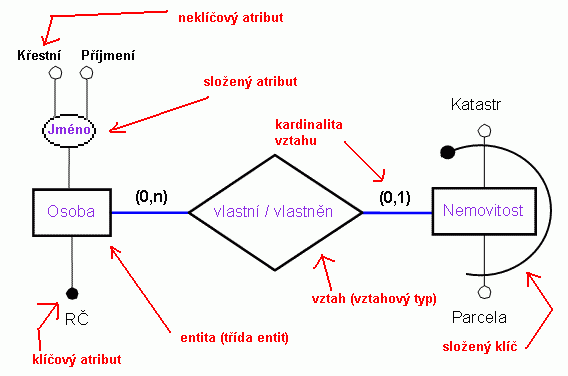
\includegraphics[width=14cm]{informatika/databazy/obrazky/er-schema.png}

(Obr�zek je upraven�, roz���en� a popsan� p��klad ze slid� Dr. T. Skopala k Datab�zov�m syst�m�m)
\end{center}
\end{obecne}

\begin{obecne}{Logick� sch�ma}
\emph{Logick� sch�ma} je datov� model organizace n�jak�ho specifick�ho celku pomoc� jednoho z datab�zov�ch model� -- podle datab�zov�ch model� popsan�ch v p�edchoz� sekci, tj. nap�. pomoc� rela�n�ch tabulek, objektov�ch t��d nebo XML. Svoj� �rovn� abstrakce se nach�z� mezi konceptu�ln�m a fyzick�m sch�matem.
\end{obecne}

\begin{obecne}{Fyzick� sch�ma}
\emph{Fyzick� datov� modely} jsou modely, ktere pou��vaj� databazov� stroje sm�rem k ni���m vrstv�m (opera�n�ho) syst�mu. V z�sad� jde o r�zn� zp�soby fyzick�ho ulo�en� dat (tedy sch�mata organizace soubor�) -- sekven�n� soubory, B-stromy apod.
\end{obecne}


%&latex
\subsection{Rela�n� datov� model, rela�n� algebra}
\begin{definiceN}{Rela�n� datov� model}
\emph{Rela�n� sch�ma} je n-tice $R(A_1: D_1, A_2: D_2, ..., A_n: D_n)$, kde mno�iny $D_i$ jsou tzv. \emph{(atributov�) dom�ny}  (odpov�d� dat.typ�m v tabulk�ch) - uv�d�j� se nepovinn�, mno�ina $A_i$ je \emph{atribut} (odpov�d� sloupci hodnot v tabulce) d�le definujme \emph{relaci} $R\subseteq A_1�A_2
... A_n$ jako mno�inu n-tic
$(a_1, a_2,...,a_n)$ (odpov�d� konktr�tn�m dat�m v tabulce) kde $a_i \in
A_i$ a \emph{prvek relace} $r\in R$ (odpov�d� ��dku v tabulce).
\end{definiceN}

\begin{prikladN}{Rela�n� datov� model}
definujeme atributy:
\begin{verbatim}
   jm�no = {Nov�k, Star�, Coufal, Li�ka}
   ulice = {Hlavn�, Severn�, Sadov�}
   m�sto = {Hradec, R�jec, Poln�}
\end{verbatim}
pak 
\begin{verbatim}
   R = {(Nov�k, Hlavn�, Harrison), (Star�, Severn�, R�jec), (Coufal, Severn�, R�jec), 
        (Li�ka, Sadov�, Poln�)}
\end{verbatim}
je relace na kart�zsk�m sou�inu (tzn. jeho podmno�ina) $jm�no � ulice � m�sto$
\\\\rela�n� sch�ma:
\begin{verbatim}
   z�kazn�k-sch�ma (jm�no:string, ulice:string, m�sto:string)
\end{verbatim}  
\end{prikladN}

\begin{definiceN}{Rela�n� algebra}
\emph{Rela�n� algebra} je mno�ina operac� (un�rn�ch, �i bin�rn�ch) na relac�ch se sch�maty, jejich� v�sledkem je op�t relace (a jej� sch�ma). 
Deklarativn� dotazovac� jazyk � tj. neprocedur�ln�, nicm�n� struktura v�razu nav�d� na po�ad� a zp�sob vyhodnocen�.
V�sledkem je v�dy kone�n� relace ��bezpe�n� definovan� operace.
\end{definiceN}

\begin{definiceN}{Operace}
Nezbytn� operace pro zachov�n� vyjad�ovac� s�ly jazyka:
\begin{pitemize}
\item \textbf{p�ejmenov�n�} - un�rn� operace, pouze se p�ejmenuj� atributy sch�matu, s daty se nic ned�je (tj. v�slekem je stejn� relace a stejn� sch�ma, pouze p��slu�n� atributy maj� jin� jm�na)
\\$R<A_i\rightarrow B_i, A_j\rightarrow B_j, ... > = <R, R((A -{A_i, A_j, ...}) \cup {B_i, B_j, ...})>$
\item \textbf{sjednocen�} - sch�mata mus� m�t stejny po�et atribut� a kompatibiln�
dom�ny
\\$<R_1, R_1(A)>\cup<R_2, R_2(A)>= <R_1\cup R_2 , R_x(A)>$
\item \textbf{rozd�l mno�in} - sch�mata mus� m�t stejny po�et atribut� a kompatibiln�
dom�ny 
\\$<R_1, R_1(A)>�<R_2, R_2(A)>= <R_1�R_2 , R_x(A)>$
\item \textbf{kart�zsk� sou�in} - vy�aduje disjuktn� schemata, pokud existuj�
stejn� jm�na atribut� mus� se nejd��ve p�ejmenovat
\\$<R_1, R_1(A)>\times<R_2, R_2(B)>= <R_1\times R_2 , R_x(\{R_1\}\times A\cup
 \{R_2\} \times B)>$
\item \textbf{selekce} - v�b�r t�ch prvk� u relace z $R$, kter� spl�uj� logickou podm�nku $\varphi(u)$ � podm�nka je zad�na Boolsk�m v�razem (tj. pomoc� spojek and, or, not) atomick�ch formul� $t_1\Theta t_2$ nebo $t_1\Theta a$, kde $\Theta \in\{<, >, =, \geq, \leq, \neq \}$ a $t_i$ jsou jm�na atribut�
\\$<R(\varphi), R(A)>= <\{u | u \in R~ \&~ \varphi(u)\}, R(A)>$
\item \textbf{projekce} - un�rn� operace, $u[C]$ je prvek relace zbaven� hodnot atribut� $A�C$, p��padn� duplicitn� prvky jsou odstran�ny
\\$<R[C], R(A)>= <\{u[C] \in R\}, R(C)>$ kde $C\subseteq A$
\end{pitemize}
Vznikl� skl�d�n�m:
\begin{pitemize}
\item \textbf{pr�nik} - sch�mata mus� m�t stejny po�et atribut� a kompatibiln�
dom�ny\\ 
$<R_1, R_1 (A)>\cap<R_2, R_2(A)>= <R_1\cap R_2 , R_x(A)>$
\\\\\\\\\\
\item \textbf{p�irozen� spojen�} - spojen� prvk� relace p�es stejn� hodnoty v�ech atribut� sd�len�ch mezi A a B, pokud $A\cap B = \oslash$, p�irozen� spojen� je vlastn� kart�zsk� sou�in (spojuje se p�es pr�zdnou mno�inu, tj. libovoln� ��v�echno se v��m�)
\\
�lze vyj�d�it pomoc� kart�zsk�ho sou�inu, selekce a projekce 
\\$<R, R(A)> * <S, S(B)>= <\{u | u[A] \in R ~\&~ u[B] \in S\}, R_x(A\cup B)>$
\\\\\\\\\\
\item \textbf{d�len�} 
$<R, R(A)> \div <S, S(B \subset A)>= <\{t | \forall s \in S (t \oplus s)\in R}, A - B\}$
\\\\\\\\\\
\end{pitemize}
TODO(respektive, je mozn�
nekter� operace formulovat pomoci ostatn�ch operaci? Kter� a jak?)
\\TODO(Formulujte predpoklady pouzitelnosti kazd� operace. Definujte
vysledek dan� operace nad relacemi.)
\end{definiceN}

\begin{poznamkaN}{Rela�n� �plnost}
Jestli�e dva v�razy ozna�uj� stejn� dotaz, jsou oba v�razy ekvivalentn�.
Dotazovac� jazyk, kter�m lze vyj�d�it v�echny konstrukce rela�n� algebry (tj. v�echny dotazy, kter� lze popsat rela�n� algebrou) se naz�v� \emph{rela�n� �pln�}.

\end{poznamkaN}

\begin{definiceN}{Rela�n� kalkulus}
Vyu�it� apar�tu predik�tov� logiky 1. ��du pro dotazov�n�. Roz���en� o �datab�zov� predik�ty, jejich� dvoj� forma definuje:
\\�dom�nov� kalkul (DRK) �pracuje s daty na �rovni atribut�
\\�n-ticov� kalkul (NRK) �pracuje s daty na �rovni n-tic (prvk� relace/��dk�)
\\\\V�sledkem dotazu v DRK / NRK je op�t relace (a jej� sch�ma).
\end{definiceN}

\begin{reportN}{IOI 10.2.2011}
a) Popi�te relacn� datov� model. Co je relacn� algebra a k cemu slouzi?\\
b) Jak� zn�te operace RA? Formulujte predpoklady pouzitelnosti kazd� operace. Definujte
vysledek dan� operace nad relacemi.\\
c) Kter� operace jsou nezbytn� pro zachovan� vyjadrovaci sily jazyka - respektive, je mozn�
nekter� operace formulovat pomoci ostatn�ch operaci? Kter� a jak?
\end{prikladN}

\begin{reportN}{IOI 21.6.2011} Co je to rela�n� algebra a jak� operace pou��v�?\\
5.2 U ka�d� operace popi�te sch�ma relace, na kter� se d� tato operace pou��t a definujte v�sledek operace.\\
5.3 Jsou v�echny operace nezbytn� pro zachov�n� vyjad�ovac� s�ly jazyka? (Pokud ne, kter� jsou?)\\
5.4 �emu odpov�d� operace p�irozen� spojen� na relac�ch, kter� maj� toto�n� sch�ma?\\
5.5 �emu odpov�d� operace p�irozen� spojen� na relac�ch, jejich� sch�mata jsou disjunktn�?
\end{prikladN}

\subsection{Algoritmy n�vrhu sch�mat relac�}


\subsubsection*{Norm�ln� formy}

\begin{obecne}{Normalizace, anom�lie}
Normalizace datab�z� je technika n�vrhu rela�n�ch datab�zov�ch tabulek, pri kter� se minimalizuj� duplicity informac� - a zamezuje se tak nekonzistentnosti dat. Stupn� normalizace se \uv{popisuj�} pomoc� \emph{norm�ln�ch forem} - ��m vy��� forma, t�m vy��� striktnost...

Probl�my �e�en� normalizac�:
\begin{pitemize}
	\item \emph{update anomaly} -- pokud se zm�n� jedna kopie redundantn�ch dat, je t�eba
zm�nit i ostatn� kopie, jinak se datab�ze stane nekonzistentn�, p�.: tabulka (�lov�k, adresa, skill); kdyby se nevykonal update spr�vn�, m��e tabulka z�stat v nekonzistentn�m stavu (nap�. by se mohly zm�nit jen n�kter� adresy jednoho �lov�ka)
	\item \emph{insertion anomaly} -- p�i vlo�en� dat p��slu�ej�c�ch jedn� entit� je pot�eba z�rove� vlo�it data i o jin� entit�, nap�. v tabulce (fakulta, datum zalo�en�, kurz) m��eme zaznamenat jen data pro fakulty, kter� maj� kurzy...
	\item \emph{deletion anomaly} -- P�i vymaz�n� dat p��slu�ej�c�ch jedn� entit� je pot�eba vymazat
data pat��c� jin� entit�. V p�edchoz� tabulce bude fakulta vymaz�na �pln�, kdy� se v�emi kurzy.
\end{pitemize}

Ide�ln� by rela�n� datab�ze m�la b�t navr�ena tak, aby vylu�ovala mo�nost takov�ch anomali�. Normalizace obvykle zahr�uje dekomponov�n� nenormalizovan� tabulky na dv� nebo v�ce tabulek takov�ch, �e po jejich spojen� (join) dostaneme v�echny p�vodn� informace.

Abychom mohli definovat norm�ln� formy, pot�ebujeme zn�t funk�n� z�vislosti jednotliv�ch atribut� entit rela�n� datab�ze a v�d�t, kter� atributy jsou kl��ov� a kter� ne.
\end{obecne}

\begin{definiceN}{Funk�n� z�vislosti}

\medskip\noindent
�ekneme, �e atribut \emph{B} je \textbf{funk�n� z�visl�} na atributu \emph{A}
(zna��me $A\rightarrow B$), jestli�e pro ka�dou hodnotu atributu \emph{A}
existuje pr�v� jedna hodnota atributu \emph{B}. Roz���en� funk�n� z�vislosti se definuj� pro mno�inu atribut� (pro ka�dou $n$-tici atribut� z n�jak� mno�iny existuje pr�v� jedna hodnota z�visl�ho(z�visl�ch) atributu(atribut�)).

Funk�n� z�vislosti spl�uj� tzv. \emph{Armstrongova pravidla}, co� zahrnuje pro mno�iny atribut� $X,Y,Z$:
\begin{penumerate}
    \item trivi�ln� z�vislost: $X\supseteq Y\ \Rightarrow\ X\to Y$
    \item transitivitu: $X\to Y \wedge Y\to Z\ \Rightarrow\ X\to Z$
    \item kompozici: $X\to Y \wedge X\to Z\ \Rightarrow X\to YZ$
    \item dekompozici: $X\to YZ \ \Rightarrow \ X\to Y \wedge X\to Z$
\end{penumerate}
\end{definiceN}

\begin{definiceN}{Kl��}
\textbf{Nadkl��em}, n�kdy t� \textbf{superkl��em}, sch�matu $A$ rozum�me ka�dou
podmno�inu mno�iny $A$, na n� $A$ funk�n� z�vis�. Jinak �e�eno nadkl�� je mno�ina
atribut�, kter� jednozna�n� ur�uje ��dek tabulky.

\textbf{Kl��}, nebo tak� \textbf{potenci�ln� kl��}(candidate key), sch�matu $A$
je takov� nadkl�� sch�matu $A$, jeho� ��dn� vlastn� podmno�ina nen� nadkl��em
$A$. �ili minim�ln� nadkl��.

Ka�d� atribut, kter� je obsa�en alespo� v jednom potenci�ln�m kl��i se naz�v�
\textbf{kl��ov�}, ostatn� atributy jsou \textbf{nekl��ov�}.
\end{definiceN}

\begin{definiceN}{Norm�ln� formy}
\begin{pitemize}
	\item \emph{Prvn� norm�ln� forma} \\ -- Tabulka je v prvn� norm�ln� form�, jestli�e lze do ka�d�ho pole dosadit pouze jednoduch� datov� typ (jsou d�le ned�liteln�). To zahrnuje i neexistenci v�ce sloupc� tabulky se stejn�m druhem obsahu:
$$
\left.\begin{aligned}
\textrm{(manager, pod��zen�1, pod��zen�2, pod��zen�3)} \\ 
\textrm{(manager, pod��zen�-vice\_hodnot\_v\_jednom\_sloupci)} \\
\end{aligned}\right\} \rightarrow \textrm{(manager, pod��zen�)}
$$
	\item \emph{Druh� norm�ln� forma} \\ 
-- Existuje kl�� a v�echna nekl��ov� pole jsou funkc� cel�ho kl��e (a tedy ne jen jeho ��st�). 
$$\textrm{(custID, name, address, city, state, zip)} \rightarrow
\begin{aligned}&\textrm{(custID, name, address, zip)}\\
&+ \textrm{(zip, city, state)}
\end{aligned}$$
	\item \emph{T�et� norm�ln� forma} \\ -- Tabulka je ve t�et� norm�ln� form�, jestli�e ka�d� nekl��ov� atribut nen� transitivn� z�visl� na ��dn�m kl��i sch�matu (resp. ka�d� nekl��ov� atribut je p��mo z�visl� na kl��i sch�matu) neboli je-li ve druh� norm�ln� form� a z�rove� neexistuje jedin� z�vislost nekl��ov�ch sloupc� tabulky. 
$$\textrm{(deptID, deptName, managerID, hireDate)} \rightarrow \textrm{(deptID, deptName, managerID)}$$
Atribut \uv{hireDate} je sice funk�n� z�visl� na kl��i deptID, ale jen proto, �e hireDate z�vis� na managerID, kter� z�vis� na deptID.
	\item \emph{Boyce-Coddova norm�ln� forma}\\ -- Pro ka�dou netrivi�ln� z�vislost $X \rightarrow Y$ plat�, �e $X$ obsahuje kl�� sch�matu $R$ ($X$ je nadkl��).
\end{pitemize}
\end{definiceN}

\subsubsection*{Algoritmy n�vrhu sch�mat relac�}

Sch�mata relac� by m�la b�t navrhov�na tak, aby odpov�dala p�edem p�ipraven�mu konceptu�ln�mu modelu (nap�. pomoc� ER diagram�) a z�rove� pokud mo�no spl�ovala co nejp��sn�j�� po�adavky na norm�ln� formy. Pro modelov�n� rela�n� datab�ze existuj� dva p��stupy:
\begin{penumerate}
    \item Z�sk�n� mno�iny rela�n�ch sch�mat (ru�n� nebo p�evodem z nap�. ER diagramu) a prov�d�n� normalizace pro ka�dou tabulku zvl᚝
    \item N�vrh tzv. univerz�ln�ho sch�matu datab�ze -- jedna velk� tabulka pro celou datab�zi (v�. platn�ch funk�n�ch z�vislost�) a normalizace prov�d�n� glob�ln�
\end{penumerate}
Prvn� mo�nost je relativn� intuitivn� (s ER diagramy) a jednoduch�, ale hroz� riziko p��li�n�ho rozdroben� datab�ze na velk� po�et mal�ch tabulek (a nadbyte�n� i vzhledem k po�adovan� norm�ln� form�). V druh�m zp�sobu jsou entity jednotliv�ch relac� \uv{vypozorov�ny} jako efekt funk�n�ch z�vislost�, co� nen� p��li� pr�hledn� a jednodu�e provediteln�, ale minimalizuje to �anci na rozdroben� datab�ze. Oba p��stupy lze tak� zkombinovat -- p�ev�st ER model datab�ze do sch�mat a n�kter� (nebo a� v�echna) potom p�ed normalizac� slou�it.

\begin{obecne}{Normalizace}
Jedin�m zp�sobem, jak u n�jak�ho obecn�ho rela�n�ho sch�matu dos�hnout norm�ln� formy (obecn� se po�aduje v�t�inou 3NF nebo BCNF), je rozd�len� na n�kolik podsch�mat. D� se to prov�st ru�n� nebo algoritmicky a existuje v�ce p��stup� podle po�adavku na norm�ln� formu, \emph{bezztr�tovost} (dekompozice relace $R( A, F )$ do $R_1(A_1,F_1)$ a $R_2(A_2,F_2)$ je bezeztr�tov�, kdy� $A1 \cap A2\to A1$ nebo $A1 \cap A2 \to A2$, tedy op�tovn�m spojen�m do p�vodn� relace nevzniknou dal�� ��dky) nebo \emph{pokryt� z�vislost�} (dekompozice $R(A,F)$ do $R_1(A_1,F_1)$ zachov�v� pokryt� z�vislost�, kdy� $F^{+}=F^{+}_1\cup F^{+}_2$ -- nesm� se ztratit z�vislost ani v r�mci d�l��ho sch�matu, ani jdouc� nap��� sch�maty).
\end{obecne}

\begin{algoritmusN}{Dekompozice}
Dekompozice je algoritmus, kter� rela�n� sch�ma p�evede do Boyce-Coddovy norm�ln� formy. Zaru�uje zachov�n� bezeztr�tovosti, ale u� ne pokryt� z�vislost� (bez ohledu na algoritmus toto u BCNF n�kdy nen� mo�n�). Jeho b�h vypad� n�sledovn�:
\begin{penumerate}
    \item Vyber n�jak� sch�ma, kter� nen� v BCNF.
    \item Vezmi pro n�j nekl��ovou z�vislost $X\to Y$ (tak �e $X$ nen� kl��) a dekomponuj podle n� -- vyho� ze sch�matu $Y$ a dej $XY$ do zvl�tn� tabulky.
    \item Opakuj od kroku 1, dokud existuje sch�ma, kter� nen� v BCNF.
\end{penumerate}
\end{algoritmusN}

\begin{algoritmusN}{Synt�za}
Algoritmus synt�zy obecn� dosahuje t�et� norm�ln� formy a zachov�v� pokryt� z�vislost� (ale ne bezeztr�tovost). Pro rela�n� sch�ma $R$ s mno�inou funk�n�ch z�vislost� $F$ vypad� n�sledovn�:
\begin{penumerate}
    \item Ud�lej minim�ln� pokryt� $F$ (vzhledem k tranzitivit�), nazvi ho $G$.
    \item Slu� funk�n� z�vislosti z $G$ se stejnou levou stranou a z ka�d� vytvo� jedno sch�ma. 
    \item Zaho� sch�mata, kter� jsou podmno�iny jin�ch.
\end{penumerate}
Nakonec je mo�n� slou�it sch�mata s funk�n� ekviv. kl��i ($K1 \leftrightarrow K2$), ale m��e to poru�it norm�ln� formu, kter� bylo dosa�eno! Pro zachov�n� bezeztr�tovosti lze do p�idat n�jak� sch�ma, obsahuj�c� univerz�ln� kl�� cel�ho p�vodn�ho (ned�len�ho) sch�matu.
\end{algoritmusN}

\begin{poznamka}
Pro nalezen� minim�ln�ho pokryt� atribut� se pou��v� pomocn� algoritmus, kter� se chov� takto:
\begin{penumerate} 
    \item Dekomponuj v�echny funk�n� z�vislosti na element�rn� (na prav� stran� je jen jeden sloupec)
    \item Odstra� z nich redundantn� atributy (takov� z lev� strany, kter� funk�n� z�vis� na jin�ch z lev� strany)
    \item Odstra� redundantn� funk�n� z�vislosti (tj. takov�, kter� jsou tranzitivn�m d�sledkem jin�ch -- prav� strana funk�n� z�vis� na lev�, i kdy� z mno�iny funk�n�ch z�vislost� onu redundantn� odstran�m)
\end{penumerate}
Pro druh� i t�et� krok je pot�eba z�skat \emph{atributov� uz�v�r} (mno�ina v�ech atribut� i tranzitivn� z�visl�ch na lev� stran�) -- to se opakovan� zkou��, jestli d�ky funk�n�m z�vislostem nedostanu z atribut� p�vodn� mno�iny n�jak� dal�� atributy (dokud nach�z�m dal��, p�id�v�m je do mno�iny a opakuji).
\end{poznamka}

\subsubsection*{Referen�n� integrita}

\begin{pitemize}
	\item pom�h� udr�ovat vztahy v rela�n� propojen�ch datab�zov�ch tabulk�ch, zabra�uje vzniku nekonzistentn�ch dat
	\item kontrola p��pustn�ch hodnot
	\item kontrola existence polo�ky s dan�m kl��em v druh� tabulce (podle ciz�ho kl��e) 
\end{pitemize}

Chov�n� p�i poru�en� integrity:
\begin{pitemize}
	\item ON UPDATE, ON DELETE - podm�nka spu�t�n� akce
	\item ON \dots RESTRICT - defaultn� �e�en� (hl�en� chyby)
	\item CASCADE - kask�dov� aktualizace/smaz�n� (sma�e p��slu�n� ��dky v odkazovan� tabulke)
	\item SET NULL - nastaven� odkazovan�ch ��dk� z�visl� tabulky na NULL
	\item SET DEFAULT - nastaven� pevn� ur�en� hodnoty
	\item NO ACTION 
\end{pitemize}

\subsection{Z�klady SQL}
TODO: p�evzato od \uv{program�tor�} z ot�zky \uv{SQL}, vzhledem k tomu, �e u n�s
se to jmenuje \uv{z�klady SQL} tak to mo�n� nemus� b�t tak podrobn�

Zdroje: slidy z p�edn�ek Datab�zov� syst�my a Datab�zov� aplikace Dr. T. Skopala a Dr. M. Kopeck�ho.

\subsubsection*{Standardy SQL}

SQL (\emph{Structured query language}) je standardn� jazyk pro p��stup k rela�n�m datab�z�m (a dotazov�n� nad nimi). Je z�rove� jazykem pro definici dat (definition data language), vytv��en� a modifikace sch�mat (tabulek), manipulaci s daty (data manipulation language), vkl��n�, aktualizace, maz�n� dat, ��zen� transakc�, definici integritn�ch omezen� aj. Jeho syntaxe odr�� snahu o co nejp�irozen�j�� formulace po�adavk� -- je podobn� anglick�m \uv{v�t�m}.

SQL je standard podle norem ANSI/ISO a existuje v n�kolika (zp�tn� kompatibiln�ch) verz�ch (ozna�ovan�ch podle roku uveden�):
\begin{description}
    \item[SQL 86] -- prvn� \uv{n�st�el}, pr�nik implementac� SQL firmy IBM
    \item[SQL 89] -- mal� revize motivovan� komer�n� sf�rou, mnoho detail� ponech�no implementaci
    \item[SQL 92] -- mnohem siln�j�� a obs�hlej�� jazyk. Zahrnuje u�
    \begin{pitemize}
	\item modifikace sch�mat, tabulky s metadaty, 
	\item vn�j�� spojen�, mno�inov� operace
	\item kask�dov� maz�n�/aktualizace podle ciz�ch kl���, transakce
	\item kurzory, v�jimky
    \end{pitemize}
    Standard existuje ve �ty�ech verz�ch: Entry, Transitional, Intermediate a Full.
    \item[SQL 1999] -- p�in�� mnoho nov�ch vlastnost�, nap�. 
    \begin{pitemize}	
	\item objektov�-rela�n� roz���en�
	\item nov� datov� typy -- reference, pole, full-text
	\item podpora pro extern� datov� soubory, multim�dia
	\item triggery, role, programovac� jazyk, regul�rn� v�razy, rekurzivn� dotazy ...
    \end{pitemize}
    \item[SQL 2003] -- dal�� roz���en�, nap�. XML management
\end{description}

Komer�n� syst�my implementuj� SQL podle r�zn�ch norem, n�kdy jenom SQL-92 Entry, dnes nej�ast�ji SQL-99, ale nikdy �pln� striktn�. N�kter� v�ci chyb� a naopak maj� v�echny spoustu nep�enositeln�ch roz���en� -- nap�. specifick� roz���en� pro procedur�ln�, transak�n� a dal�� funkcionalitu (T-SQL (Microsoft SQL Server), PL-SQL (Oracle) ). S nov�mi verzemi se kompatibilita zlep�uje, �asto je mo�n� pou��vat oboj� syntax. P�enos aplikace za b�hu na jinou platformu je ale st�le velice n�ro�n� -- a to t�m n�ro�n�j��, ��m v�c v�c� mimo SQL-92 Entry obsahuje.Pro otestov�n�, zda je �patn� syntax SQL, nebo zda jen dan� datab�zov� platforma nepodporuje n�kter� prvek, slou�� SQL valid�tory (kter� testuj� SQL podle norem.


\subsubsection*{Dotazy v SQL}

Hlavn�m n�strojem dotaz� v SQL je p��kaz \texttt{SELECT}. Sd�l� prvky rela�n�ho kalkulu i rela�n� algebry -- obsahuje pr�ci se sloupci, kvantifik�tory a agrega�n� funkce z rela�n�ho kalkulu a dal�� operace -- projekce, selekce, spojen�, mno�inov� operace -- z rela�n� algebry. Na rozd�l od striktn� formulace rela�n�ho modelu datab�ze povoluje duplik�tn� ��dky a NULLov� hodnoty atribut�.

Net��d�n� dotaz v SQL sest�v� z:
\begin{pitemize}
    \item p��kazu(�) \texttt{SELECT} (hlavn� logika dotazov�n�), to obsahuje v�dy
    \item m��e obsahovat i mno�inov� operace nad v�sledky p��kaz� \texttt{SELECT} -- \texttt{UNION}, \texttt{INTERSECTION} ...
\end{pitemize}
V�sledky nemaj� definovan� uspo��d�n� (resp. jejich po�ad� je ur�eno implementac� vyhodnocen� dotazu).

P��kaz \texttt{SELECT} vypad� n�sledovn� (tato verze u� zahrnuje i t��d�n� v�sledk�):
\begin{verbatim}
SELECT [DISTINCT]
 v�raz1 [[AS] c_alias1] [, ...]
FROM
 zdroj1 [[AS] t_alias1] [, ...]
[WHERE podm�nka_�]
[GROUP BY v�raz_g1 [, �]
[HAVING podm�nka_s]]
[ORDER BY v�raz_o1 [, �] ASC/DESC]
\end{verbatim}
Kde
\begin{pitemize}
    \item v�razy mohou b�t sloupce, sloupce s agrega�n�mi funkcemi, v�sledky dal��ch funkc� ...

\noindent \texttt{ v�raz = <n�zev sloupce>, <konstanta>, \\
 (DISTINCT) COUNT(~<n�zev sloupce>~),\\
{}[DISTINCT] [~SUM~|~AVG~](~<v�raz>~),\\
{}[~MIN~|~MAX~](~<v�raz>~)}\\
a nav�c lze pou��t oper�tory $+,-,*,/$.

    \item zdroje jsou tabulky nebo vno�en� selecty
    \item v�razy i zdroje b�t p�ejmenov�ny pomoc� \texttt{AS}, nap�. pro odkazov�n� uvnit� dotazu nebo jm�na na v�stupu (od SQL-92)
    \item podm�nka je logick� podm�nka (spojovan� logick�mi spojkami \texttt{AND, OR}) na hodnoty dat ve zdroj�ch:

\texttt{podm�nka = <v�raz> BETWEEN <x> AND <y>, <v�raz> LIKE "\%\_ ... ",\\
<v�raz> IS [NOT] NULL,\\
<v�raz> > = <> <= < > [<v�raz>/ ALL / ANY <dotaz>],\\
<v�raz> NOT IN [<seznam hodnot> / <dotaz>], EXIST ( <dotaz> )}

    \item \texttt{GROUP BY} znamen� agregaci podle unik�tn�ch hodnot jmenovan�ch sloupc� (v ostatn�ch sloupc�ch vznikaj� mno�iny hodnot, kter� se spolu s on�mi unik�tn�m� vyskytuj� na stejn�ch ��dk�ch
    \item \texttt{HAVING} ozna�uje podm�nku na agregaci
    \item \texttt{ORDER BY} definuje, podle hodnot ve kter�ch sloupc�ch nebo podle kter�ch jin�ch v�raz� nad nimi proveden�ch se m� v�sledek set��dit (\texttt{ASC} po�aduje vzestupn� set��d�n�, \texttt{DESC} sestupn�).
\end{pitemize}

SQL nem� p��kaz na omezen� rozsahu na n�kter� ��dky (jako nap�. \uv{pot�ebuji jen 50.-100. ��dek v�pisu}), a to lze �e�it bu� slo�it� standardn� (po��t�n� kolik hodnot je men��ch ne� vybran�, nav�c n�ro�n� na hardware) nebo pomoc� n�kter�ho nep�enositeln�ho roz���en�.

\medskip\noindent
Po�ad� vyhodnocov�n� jednoho p��kazu \texttt{SELECT} (nebereme v �vahu optimalizace):
\begin{penumerate}
    \item Nejprve se zkombinuj� data ze v�ech zdroj� (tabulek, pohled�, poddotaz�). Pokud jsou odd�leny ��rkami, provede se kart�zsk� sou�in (to sam� co \texttt{CROSS JOIN}), v SQL-92 a vy���m i slo�it�j�� spojen� -- \texttt{JOIN ON} (vnit�n� spojen� podle podm�nky), \texttt{NATURAL JOIN} (\uv{p�irozen�} spojen� podle stejn�ch hodnot stejn� pojmenovan�ch sloupc�), \texttt{OUTER JOIN} (\uv{vn�j��} spojen�, do kter�ho jsou zahrnuty i z�znamy, pro kter� v jednom ze zdroj� nen� nalezeno nic, co by odpov�dalo podm�nce, dopln�nn� NULLov�mi hodnotami) atd.
    \item Vy�ad� se vznikl� ��dky, kter� nevyhovuj� podm�nce (\texttt{WHERE})
    \item Zbyl� ��dky se seskup� do skupin se stejn�mi hodnotami uveden�ch v�raz� (\texttt{HAVING}), ka�d� skupina obsahuje atomick� sloupce s hodnotami uveden�ch v�raz� a mno�inov� sloupce se skupinami ostatn�ch hodnot sloupc�.
    \item Vy�ad� se skupiny, nevyhovuj�c� podm�nce (\texttt{HAVING})
    \item V�sledky se set��d� podle po�adavk�
    \item Vygeneruje se v�stup s po�adovan�mi hodnotami
    \item V p��pad� \texttt{DISTINCT} se vy�ad� duplicitn� ��dky
\end{penumerate}


\begin{e}{Pozn�mka}{0}{0}
\begin{pitemize}
    \item Klauzule \texttt{GROUP BY} set��d� p�ed vytvo�en�m skupin v�echny ��dky dle v�raz� v klauzuli. Proto by se m�l seskupovat co nejmen�� mo�n� po�et ��dek. Pokud je mo�n� ��dky odfiltrovat pomoc� WHERE, je v�sledek efektivn�j��, ne� n�sledn� odstra�ov�n� cel�ch skupin.
    \item  Klauzule \texttt{DISTINCT} t��d� v�sledn� z�znamy (p�ed operac� ORDER BY), aby na�la duplicitn� z�znamy. Pokud to jde, je vhodn� se bez n� obej�t.
    \item Klauzule \texttt{ORDER BY} by m�la b�t pou�ita jen v nutn�ch p��padech. Nen� p��li� vhodn� ji pou��vat v definic�ch pohled�, nad kter�mi se d�le d�laj� dal�� dotazy
\end{pitemize}
\end{e}


\subsubsection*{Definice a manipulace s daty, ostatn� p��kazy}

Standard SQL podporuje n�kolik druh� datov�ch typ�:
\begin{pitemize}
    \item textov� v n�rodn� a glob�ln� (UTF) znakov� sad� (n�kolika druh� -- prom�nn� a pevn� d�lky): \texttt{CHARACTER(n)}, \texttt{NCHAR(n)},
    \texttt{CHAR VARYING(n)}
    \item ��seln� typy -- \texttt{ NUMERIC(p[,s]), INTEGER, INT, SMALLINT,\\  FLOAT(presnost), REAL, DOUBLE PRECISION}
    \item datumov� typy -- \texttt{DATE, TIME, TIMESTAMP, TIMESTAMP(presnost\_sekund) WITH TIMEZONE}
\end{pitemize}
Datab�zov� servery ne v�dy podporuj� v�echny uveden� typy. Nemus� je podporovat nativn�, n�kdy si pouze \uv{p�elo��} n�zev typu na podobn� nativn� podporovan� typ.

\medskip
\begin{obecne}{P��kaz \texttt{CREATE TABLE}}
Tento p��kaz slou�� k vytvo�en� nov� tabulky. Je nutn� definovat jej� n�zev, atributy a jejich dom�ny (datov� typy); d�le je mo6n� definovat integritn� omezen� (kl��e, ciz� kl��e, odkazy, podm�nky). P��kaz vypad� n�sledovn�:
\begin{center}
\texttt{CREATE TABLE <n�zev> <def. sloupce/i.o. tabulky, ...> }
\end{center}
A uvnit� potom
\begin{verbatim}
def. sloupce = <n�zev> <dat.typ> 
    [DEFAULT NULL|<hodnota>] [<i.o.sloupce>] 
dat.typ = [VARCHAR(n) | BIT(n) | INTEGER | FLOAT | DECIMAL ...] 
i.o.sloupce = [CONSTRAINT <jm�no>] [NOT NULL / UNIQUE / PRIMARY KEY], 
    REFERERENCES <tabulka>(<sloupec>) <akce>, CHECK <podm�nka> 
akce = [ON UPDATE / ON DELETE] 
    [CASCADE / SET NULL / SET DEFAULT / NO ACTION(hl�en� chyby) ] 
i.o.tabulky = UNIQUE, PRIMARY KEY <sloupec, ... >, 
    FOREIGN KEY <sloupec, ... >, 
    REFERENCES <tabulka>(<sloupec, ... >), 
    CHECK( <podm�nka> )
\end{verbatim}
\end{obecne}

\medskip
\begin{obecne}{P��kazy pro manipulaci se sch�matem}
\begin{pitemize}
    \item �prava tabulky:
\begin{verbatim}
ALTER TABLE <n�zev> ADD {COLUMN} <def.sloupce>, ADD <i.o.tabulky>, 
    ALTER COLUMN <sloupec> [ SET / DROP ], DROP COLUMN <sloupec>, 
    DROP CONSTRAINT <jm�no i.o.> 
\end{verbatim}
    \item Smaz�n� tabulky (nen� to sam� jako vymaz�n� v�ech dat z tabulky!):
\begin{verbatim}
DROP TABLE <tabulka> 
\end{verbatim}
    \item Vytvo�en� \uv{pohledu} -- navenek se chov� jako tabulka, ale vnit�n� se p�i ka�d�m dotazu provede vno�en� dotaz (kter� definic� pohledu zapisuji):
\begin{verbatim}
CREATE VIEW <n�zev "tabulky"> ( <sloupec, ... > ) 
    AS <dotaz> {WITH [ LOCAL / CASCADED ] CHECK OPTION }
\end{verbatim}
    N�kter� datab�zov� platformy umo��uj� do takto vytvo�en�ch pohled� i zapisovat.
\end{pitemize}
\end{obecne}

\medskip
\begin{obecne}{P��kazy pro manipulaci s daty}
\begin{pitemize}
    \item Vlo�en� nov�ch dat do tabulky
\begin{verbatim}
INSERT INTO <tabulka> ( <sloupec, ... > ) 
    [VALUES ( <v�raz, ... > ) / (<dotaz>) ] 
\end{verbatim}
    \item �prava dat (na ��dc�ch kter� vyhovuj� podm�nce se nastav� zadan� hodnoty vybran�m sloupc�m):
\begin{verbatim}
UPDATE <tabulka> SET 
    ( <sloupec> = [ NULL / <v�raz> / <dotaz> ] , ... ) 
    WHERE (<podm�nka>) 
\end{verbatim}
    \item Smaz�n� ��dk� vyhovuj�c�ch podm�nce z tabulky:
\begin{verbatim}
DELETE FROM <tabulka> ( WHERE <podm�nka> ) 
\end{verbatim}
\end{pitemize}
\end{obecne}

\subsection{Transakční zpracování, vlastnosti transakcí, uzamykací protokoly, zablokování}

\begin{definiceN}{Transakce}
\emph{Transakce} je jistá posloupnost nebo specifikace posloupnosti akcí práce s databází, jako
jsou čtení, zápis nebo výpočet, se kterou se zachází jako s jedním celkem.
\end{definiceN}

Hlavním smyslem používání transakcí, tj. \emph{transakčního zpracování}, je
udržení databáze v konzistentním stavu. Jestliže na sobě některé operace závisí,
sdružíme je do jedné transakce a tím zabezpečíme, že budou vykonány buď
všechny, nebo žádná. Databáze tak před i po vykonání transakce bude v
konzistentním stavu. Aby se uživateli transakce jevila jako jedna atomická
operace, je nutné zavést příkazy COMMIT a ROLLBACK. První z nich signalizuje
databázi úspěšnost provedení transakce, tj. veškeré změny v databázi se stanou
trvalými a jsou zviditelněny pro ostatní transakce, druhý příkaz signalizuje
opak, tj. databáze musí být uvedena do původního stavu.

Tyto příkazy většinou není nutné volat explicitně, např. příkaz COMMIT je vyvolán po
normálním ukončení programu realizujícího transakci. Příkaz ROLLBACK pro svou
funkci vyžaduje použití tzv. \emph{žurnálu} (logu) na nějakém stabilním
paměťovém médiu. Žurnál obsahuje historii všech změn databáze v jisté časové
periodě.

Jednoduchá transakce vypadá většinou takto:
\begin{penumerate}
  \item Začátek transakce,
  \item provedení několika dotazů -- čtení a zápisů (žádné změny v databázi nejsou zatím vidět pro
  okolní svět),
  \item Potvrzení (příkaz COMMIT) transakce (pokud se transakce povedla, změny
  v databázi se stanou viditelné).
\end{penumerate}
Pokud nějaký z provedených dotazů selže, systém by měl celou transakci zrušit a
vrátit databázi do stavu v jakém byla před zahájením transakce (operace ROLLBACK).

Transakční zpracování je také ochrana databáze před hardwarovými nebo
softwarovými chybami, které mohou zanechat databázi po částečném zpracování
transakce v nekonzistentním stavu. Pokud počítač selže uprostřed provádění
některé transakce, transakční zpracování zaručí, že všechny operace z
nepotvrzených (\uv{uncommitted}) transakcí budou zrušeny. 

\subsubsection*{Vlastnosti transakcí}

Podívejme se nyní na vlastnosti požadované po transakcích. Obvykle se používá
zkratka prvních písmen anglických názvů vlastností \textbf{ACID}~-- atomicity,
consistency, isolation (independence), durability. 
\begin{description}
  \item[atomicita] -- transakce se tváří jako jeden celek, musí buď proběhnout
  celá, nebo vůbec ne.
  \item[konzistence] -- transakce transformuje databázi z jednoho konzistentního
  stavu do jiného konzistentního stavu.
  \item[nezávislost] -- transakce jsou nezávislé, tj. dílčí efekty transakce
  nejsou viditelné jiným transakcím.
  \item[trvanlivost] -- efekty úspěšně ukončené (potvrzené,\uv{commited})
  transakce jsou nevratně uloženy do databáze a nemohou být zrušeny.
\end{description}

Transakce mohou být v uživatelských programech prováděny paralelně (spíše
zdánlivě paralelně, stejně jako je paralelismus multitaskingu na jednoprocesorových
strojích jen zdánlivý, zajistí to ale možnost paralelizace \uv{nedatabázových} 
akcí a pomalé transakce nebrzdí rychlé). Je
zřejmé, že posloupnost transakcí může být zpracována paralelně různým způsobem.
Každá transakce se skládá z několika akcí. Stanovené pořadí provádění akcí
více transakcí v čase nazveme \textbf{rozvrhem}.

Rozvrh, který splňuje následující podmínky, budeme nazývat \textbf{legální}:
\begin{pitemize}
  \item Objekt je nutné mít uzamknutý, pokud k němu chce transakce přistupovat.
  \item Transakce se nebude pokoušet uzamknout objekt již uzamknutý jinou
  transakcí (nebo musí počkat, než bude objekt odemknut).
\end{pitemize}

Důležitými pojmy pro paralelní zpracování jsou sériovost či uspořádatelnost.
\textbf{Sériové rozvrhy} zachovávají operace každé transakce pohromadě (a 
provádí se jen jedna transakce najednou). Pro $n$
transakcí tedy existuje $n!$ různých sériových rozvrhů. Pro získání korektního
výsledku však můžeme použít i rozvrhu, kde jsou operace různých transakcí
navzájem prokládány.
Přirozeným požadavkem na korektnost je, aby efekt paralelního zpracování
transakcí byl týž, jako kdyby transakce byly provedeny v nějakém sériovém rozvrhu.
Předpokládáme-li totiž, že každá transakce je korektní program, měl by vést
výsledek sériového zpracování ke konzistentnímu stavu. O systému zpracování
transakcí, který zaručuje dosažení konzistentního stavu nebo stejného stavu
jako sériové rozvrhy, se říká, že zaručuje \textbf{uspořádatelnost}.

Mohou se vyskytnout problémy, které uspořádatelnosti zamezují. Ty nazýváme \emph{konflikty}. Plynou z pořadí dvojic akcí různých transakcí na stejném objektu. Existují tři typy konfliktních situací:
\begin{penumerate}
    \item WRITE-WRITE -- přepsání nepotvrzených dat
    \item READ-WRITE -- neopakovatelné čtení
    \item WRITE-READ -- čtení nepotvrzených (\uv{uncommitted}) dat
\end{penumerate}

Řekneme, že rozvrh je \emph{konfliktově uspořádatelný}, je-li konfliktově ekvivalentní nějakému sériovému rozvrhu (tedy jsou v něm stejné, tj. žádné konflikty). Test na konfliktovou uspořádatelnost se dá provést jako test acykličnosti grafu, ve kterém konfliktní situace představují hrany a transakce vrcholy. Konfliktová uspořádatelnost je slabší podmínka než uspořádatelnost -- nezohledňuje ROLLBACK (\emph{zotavitelnost} -- zachování konzistence, i když kterákoliv transakce selže) a dynamickou povahu databáze (vkládání a mazání objektů). Zotavitelnosti se dá dosáhnout tak, že každá transakce $T$ je potvrzena až poté, co jsou potvrzeny všechny ostatní transakce, které změnily data čtená v $T$. Pokud v zotavitelném rozvrhu dochází ke čtení změn pouze potvrzených transakcí, nemůže dojít ani k jejich \emph{kaskádovému rušení}.

Při zpracování (i uspořádatelného) rozvrhu může dojít k situaci \emph{uváznutí} -- \emph{deadlocku}. To nastane tehdy, pokud jedna transakce $T_1$ čeká na zámek na objekt, který má přidělený $T_2$ a naopak. Situaci lze zobecnit i na více transakcí. Uváznutí lze buď přímo zamezit charakterem rozvrhu, nebo detekovat (hledáním cyklu v grafu čekajících transakcí, tzv. \uv{waits-for} grafu) a jednu z transakcí \uv{zabít} a spustit znova.

\medskip
K zajištění uspořádatelnosti a zotavitelnosti a zabezpečení proti kaskádovým rollbackům a deadlocku se používají různá schémata (požadavky na rozvrhy). Jedním z nich jsou uzamykací protokoly.

\subsubsection*{Uzamykací protokoly}

Vytváření rozvrhů a testování jejich uspořádatelnosti není pro praxi zřejmě ten
nejvhodnější způsob. Pokud ale budeme transakce konstruovat podle určitých
pravidel, tak za určitých předpokladů bude každý jejich rozvrh uspořádatelný.
Soustavě takových pravidel se říká \textbf{protokol}.

Nejznámější protokoly jsou založeny na dynamickém zamykání a odemykání objektů v
databázi. Zamykání (operace LOCK) je akce, kterou vyvolá transakce na objektu,
aby ho chránila před přístupem ostatních transakcí.

\begin{definiceN}{Dobře formovaná transakce}
Transakci nazveme \textbf{dobře formovanou} pokud podporuje přirozené požadavky
na transakce:
\begin{penumerate}
  \item transakce zamyká objekt, chce-li k němu přistupovat,
  \item transakce nezamyká objekt, který již je touto transakcí uzamčený,
  \item transakce neodmyká objekt, který není touto transakcí zamčený,
  \item po ukončení transakce jsou všechny objekty uzamčené touto transakcí
  odemčeny.
\end{penumerate}
\end{definiceN}

\paragraph{Dvoufázový protokol (2PL)} -- Dvoufázová transakce v první fázi
zamyká vše co je potřeba a od prvního odemknutí (druhá fáze) již jen odemyká co
měla zamčeno (již žádná operace LOCK). Tedy transakce musí mít všechny objekty
uzamčeny předtím, než nějaký objekt odemkne. Dá se dokázat, že pokud jsou
všechny transakce v dané množině transakcí dobře formované a dvoufázové, pak
každý jejich legální rozvrh je uspořádatelný.

Dvoufázový protokol zajišťuje uspořádatelnost, ale ne zotavitelnost ani
bezpečnost proti kaskádovému rušení transakcí nebo uváznutí.

\paragraph{Striktní dvoufázový protokol (S2PL)} -- Problémy 2PL jsou nezotavitelnost
a kaskádové rušení transakcí. Tyto nedostatky lze odstranit pomocí striktních
dvoufázových protokolů, které uvolňují zámky až po skončení transakce (COMMIT).
Zřejmá nevýhoda je omezení paralelismu. 2PL navíc stále nevylučuje možnost deadlocku.

\paragraph{Konzervativní dvoufázový protokol (C2PL)} -- Rozdíl oproti 2PL je
ten, že transakce žádá o všechny své zámky, ještě než se začne
vykonávat. To sice vede občas k zbytečnému zamykání (nevíme co přesně budeme
potřebovat, tak radši zamkneme víc), ale stačí to již k prevenci uváznutí
(deadlocku).

\subsubsection*{\uv{Vylepšení} zamykacích protokolů}

\paragraph{Sdílené a výlučné zámky} -- Nevýhodou 2PL je, že objekt může mít
uzamčený pouze jedna transakce. Abychom uzamykání provedli precizněji, je dobré
vzít na vědomí rozdíl mezi operacemi READ a WRITE. \emph{Výlučný zámek}
(W\_LOCK) může být aplikován na objekty jak pro operaci READ tak pro WRITE,
\emph{sdílený zámek} (R\_LOCK) uzamyká objekt, který chceme pouze číst. Jeden
objekt potom může být uzamčen sdíleným zámkem více transakcí a zvyšuje se tak
možnost paralelního zpracování. Budeme-li s těmito zámky zacházet stejně jako u
2PL, opět máme zaručenou uspořádatelnost rozvrhu, ovšem nikoliv absenci uváznutí.


\paragraph{Strukturované uzamykání (multiple granularity)} -- Objekty jsou v
tomto případě chápány hierarchicky dle relace \emph{obsahuje}. Například
databáze obsahuje soubory, které obsahují stránky a ty zase obsahují jednotlivé
záznamy. Na tuto hierarchii se můžeme dívat jako na strom, ve kterém každý
vrchol obsahuje své potomky. Když transakce zamyká objekt (vrchol) zamyká také
všechny jeho potomky. Protokol se tak snaží minimalizovat počet zámků, tím
snížit režii a zvýšit možnosti paralelního zpracování.


\subsubsection*{Alternativní protokoly}

\paragraph{Časová razítka} -- Další z protokolů zaručující uspořádatelnost je
využití časových razítek. Na začátku dostane transakce $T$ \emph{časové
razítko}~-- $TS(T)$ (časová razítka jsou unikátní a v čase rostou), abychom věděli
pořadí, ve kterém by měli být transakce vykonány. Každý objekt v databázi má
\emph{čtecí razítko}~-- $RTS(O)$ (read timestamp), které je aktualizováno, když je
objekt čten, a \emph{zapisovací razítko}~-- $WTS(O)$ (write timestamp), které je
aktualizováno, když nějaká transakce objekt mění.

Pokud chce transakce $T$ číst objekt $O$ mohou nastat dva případy:
\begin{pitemize}

  \item $TS(T) < WTS(O)$, tzn. někdo změnil objekt $O$ potom co byla spuštěna
  transakce $T$. V tomto případě musí být transakce zrušena a spouštěna znovu (a
  tedy s jiným časovým razítkem).

  \item $TS(T) > WTS(O)$, tzn. je bezpečné objekt číst. V tomto případě $T$
  přečte $O$ a $RTS(O)$ je nastaveno na $\max\{TS(T),\ RTS(O)\}$.

\end{pitemize}

Pokud chce transakce $T$ zapisovat do objektu $O$ rozlišujeme případy tři:
\begin{pitemize}

  \item $TS(T) < RTS(O)$, tzn. někdo četl $O$ poté co byla spuštěna $T$ a
  předpokládáme, že si pořídil lokální kopii. Nemůžeme tedy $O$ změnit, protože
  by lokální kopie přestala být platná a tedy je nutné $T$ zrušit a spustit
  znova.

  \item $TS(T) < WTS(O)$, tzn. někdo změnil $O$ po startu $T$. V tomto případě
  přeskočíme write operaci a pokračujeme dále normálně. $T$ nemusí být
  restartována.

  \item V ostatních případech $T$ změní $O$ a $WTS(O)$ je nastaveno na $TS(T)$.
\end{pitemize}

\paragraph{Optimistické protokoly} -- V situaci kdy se většina transakcí
neovlivňuje, je režie výše uvedených protokolů zbytečně velká a můžeme použít
takzvaný optimistický protokol. V protokolu můžeme rozlišit tři fáze.
\begin{penumerate}

  \item \textbf{Fáze čtení:} Čtou se objekty z databáze do lokální paměti a jsou
  na nich prováděny potřebné změny.

  \item \textbf{Fáze kontroly:} Po dokončení všech změn v lokální paměti je
  vyvolán pokus o zapsání výsledků do databáze. Algoritmus zkontroluje, zda
  nehrozí potenciální kolize s již potvrzenými transakcemi, nebo s některými
  právě probíhajícími. Pokud konflikt existuje, je třeba spustit algoritmus pro
  řešení kolizí, který se je snaží vyřešit. Pokud se mu to nepodaří, je využita
  poslední možnost a tou je zrušení a restartování transakce.

  \item \textbf{Fáze zápisu:} Pokud nehrozí žádné konflikty, jsou data z lokální
  paměti zapsány do databáze a transakce potvrzena.

\end{penumerate}




\subsection{Organizace dat na vn�j�� pam�ti, B-stromy a jejich varianty}


\subsubsection*{Vn�j�� pam�}

\begin{e}{Definice}{0}{Vn�j�� pam�}
\emph{Vn�j�� pam�} je �lo�i�t� dat (pam�ov� m�dium), u kter�ho je rychlost na��t�n� dat zpravidla n�zk� a p��stup k nim ne �pln� p��m� (z�le�� na uspo��d�n� dat na m�diu), ne-li pouze sekven�n� (oproti vnit�n� pam�ti s rychl�m n�hodn�m p��stupem a men�� kapacitou). P��kladem vn�j�� pam�ti je pevn� disk nebo magnetick� p�ska.

\emph{Magnetick� p�sky} poskytuj� vysokou kapacitu, ale n�zkou rychlost a pouze sekven�n� p��stup. Pro jejich kapacitu je d�le�it� hustota z�znamu, pot�ebuj� meziblokov� mezery pro vyrovn�n� nep�esnosti p�et��en� p�sky.

\emph{Pevn� disky} umo��uj� p��m� p��stup, ale jeho rychlost nen� v�dy stejn�. Ovliv�uje ji fyzick� vzd�lenost dat -- pevn� disk m� n�kolik \emph{v�lc�}, na nich� jsou ulo�eny jednotliv� datov� \emph{stopy}. K v�lc�m p��slu�� \emph{�tec� hlavy} (je jich stejn� jako v�lc�, ale pohybuj� se v�echny sou�asn�, tak�e m��e v 1 okam�iku ��st jen jedna). Disky jsou v�t�inou rozd�leny na \emph{sektory} -- nejmen�� jednotku dat, kterou je mo�n� na��st nebo ulo�it (zpravidla jednotky KB). Pro rychlost p��stupu k dat�m jsou d�le�it� tyto veli�iny (v�robcem disk� jsou zpravidla ud�v�ny pr�m�rn� hodnoty):
\begin{pitemize}
    \item \emph{seek} ($s$) -- p�esun na jinou stopu, dnes zpravidla kolem 4-8~ms
    \item \emph{(average) rotational delay} ($r$) -- oto�en� v�lc� -- 1 p�lot��ka, pro nej�ast�j�� 7200rpm disk je to cca 4~ms
    \item \emph{block transfer time} ($btt$) -- doba p�enesen� 1 bloku po sb�rnici, na ATA/100 disku se 4~KB bloky teoreticky 0.04~ms
\end{pitemize}
Pokud jsou data um�st�na na disku za sebou sekven�n�, rychlost jejich na�ten� je mnohem vy��� ne� p�i n�hodn�m rozm�st�n�, proto�e nen� t�eba prov�d�t p�esuny mezi stopami a ot��en� v�lc� nav�c.
\end{e}

\begin{e}{P��klad}{0}{0}
\emph{Jak vypad� na�ten� 1~MB dat z pevn�ho disku?} P�edpokl�dejme, �e na 1 stopu se vejde 512~KB a 1 blok m� 4~KB. Jsou-li data um�st�na na disku sekven�n�, pot�ebuji pro na�ten� 1~MB dat naj�t prvn� blok a potom ��st dv� cel� stopy (2 ot��ky), tj. celkem $s+r+(2\cdot2r)$ (a p�enos po sb�rnici lze zanedbat, proto�e prob�h� z�rove� se �ten�m). Pokud jsou data na disku n�hodn� rozprost�ena, pot�ebuji celkem 256-kr�t naj�t blok a na��st ho: $256\cdot(s+r+btt)$, tak�e operace trv� a� 100-kr�t d�le.
\end{e}


\subsubsection*{Soubor}

\begin{e}{Definice}{0}{Z�znam, kl��}
\emph{(Logick�) z�znam} je jednotka dat (nap�. v datab�zi), m� \emph{atributy} (z nich� ka�d� m� jm�no a dom�nu -- povolenou mno�inu hodnot). Logick�mu z�znamu v reprezentaci na disku odpov�d� \emph{fyzick� z�znam} (n�jak� d�lky $R$ -- pevn� nebo prom�nn�), kter� nav�c m��e obsahovat je�t� dal�� data -- odd�lova�e, ukazatele, hlavi�ky. 

\emph{Kl��} je mno�ina atribut�, kter� jednozna�n� identifikuje z�znam; proti tomu \emph{vyhled�vac� kl��} je mno�ina atribut�, pro kterou lze nal�zt mno�inu odpov�daj�c�ch z�znam�. Vyhled�vac� kl��e jsou t�� druh�: hodnotov� (\uv{oby�ejn�} hodnoty n�kter�ch atribut�), ha�ovan� a relativn� (p��mo pozice v souboru).
\end{e}

\begin{e}{Definice}{0}{Soubor}
(Homogenn�) \emph{soubor} je multimno�ina z�znam�. Fyzicky na vn�j�� pam�ti je organizov�n do \emph{blok� (str�nek)} (velikosti $B$, typicky n�kolika KB) -- hl. jednotkou p�enosu dat mezi vnit�n� a vn�j�� pam�t�. Pom�r velikosti z�znamu k velikosti bloku ($B/R$) se naz�v� \emph{blokovac� faktor} ($\lfloor b\rfloor$). Z�znamy mohou b�t rozprost�eny i p�es n�kolik str�nek, nebo m��e b�t pouze jeden z�znam na 1 str�nku; ide�ln� (ale ne v�dy dosa�iteln�) je, pokud beze zbytku zapl�uj� str�nky. Na souboru jsou definov�ny operace se z�znamy: \emph{insert, delete, update} a \emph{fetch}.
\end{e}

\begin{e}{Definice}{0}{Dotaz}
\emph{Dotaz} je ka�d� funkce, kter� ka�d�mu sv�mu argumentu p�i�ad� odpov�daj�c� mno�inu z�znam� ze souboru (\uv{tot�ln� vy��sliteln� funkce definovan� na souboru}). Dotazy mohou b�t t�chto typ�:
\begin{pitemize}
    \item Na�ten� v�ech z�znam� ({\tt SELECT * FROM tabulka})
    \item Na �plnou shodu ({\tt SELECT * FROM tabulka WHERE sloupec1 = 'hodnota' AND sloupec2 = 'hodnota'} pro tabulku se 2 sloupci -- d�ny jsou v�echny atributy)
    \item Na ��ste�nou shodu\\({\tt SELECT * FROM tabulka WHERE sloupec1 = 'hodnota'} pro tabulku se 2 sloupci -- zadan� je jen ��st atribut�)
    \item Na intervalovou shodu (��ste�nou nebo �plnou) ({\tt SELECT * FROM tabulka WHERE sloupec1 > 'hodnota'})
\end{pitemize}
U soubor� se sleduje rychlost proveden� t�chto operac�.
\end{e}


\subsubsection*{Statick� metody organizace souboru}

\begin{e}{Definice}{0}{Sch�ma organizace souboru}
\emph{Sch�ma organizace souboru} je popis logick� pam�ov� struktury, do n� lze zobrazit logick� soubor, spolu s algoritmy operac� nad touto strukturou. Ta je obvykle tvo�ena z logick�ch str�nek (blok� pevn� d�lky) a m��e popisovat v�ce prov�zan�ch log. soubor�, z nich� \emph{prim�rn� soubor} je ten, kter� obsahuje u�ivatelsk� data. Operace definovan� nad sch�matem org. souboru jsou krom� operac� nad soubory je�t� \emph{build, reorganization, open} a \emph{close}.

Proti n�mu stoj� \emph{fyzick� sch�ma souboru} -- struktura nad fyzick�mi soubory, nejbl�e hardwaru je \emph{implementa�n� sch�ma souboru}.

Zaji�t�n� \emph{Vyv�enosti struktury} znamen� zaji�t�n� omezen� cesty p�i vyhled�v�n� n�jak�m v�razem (zaru�en� asymptotick� slo�itosti), nav�c zaru�en� rovnom�rnosti zapln�n� struktury -- \emph{faktor napln�n� str�nek}. Sch�mata, kter� spl�uj� ob� podm�nky, se naz�vaj� \emph{dynamick�}, ostatn� jsou ozna�ov�na jako \emph{statick�}.
\end{e}

\begin{e}{Pozn�mka}{0}{�asov� odhady}
Pro sch�mata organizace soubor� se po��taj� �asov� odhady proveden� jednotliv�ch operac� -- jednodu���ch, jako je p��stup k z�znamu ($T_F$), \emph{rewrite} -- p�epis b�hem 1 ot��ky disku ($T_{RW}$), p��p. sekven�n� �ten�; d�le i slo�it�j��ch jako vyhled�n� z�znamu, p�id�n�, smaz�n� a �prava z�znamu, reorganizace struktury nebo na�ten� cel�ho souboru.
\end{e}

\begin{obecne}{Hromada (neuspo��dan� sekven�n� soubor)}
\emph{Hromada(heap)} je naprosto nejjednodu��� sch�ma organizace souboru, kdy jsou z�znamy v souboru jen n�hodn� se�azeny za sebou. �asov� slo�itost vyhled�v�n� je $O(n)$, pokud $n$ je po�et z�znam�. Jde o \emph{nehomogenn� soubor}, kde z�znamy obvykle nemaj� pevnou d�lku. 
\end{obecne}

\begin{obecne}{Uspo��dan� sekven�n� soubor}
V \emph{uspo��dan�m sekven�n�m souboru} jsou z�znamy �azeny podle kl��e. Aktualizovan� z�znamy se um�st� do zvl�tn�ho souboru a a� p�i dal�� operaci \uv{reorganization} jsou p�id�ny do prim�rn�ho. Slo�itost nalezen� z�znamu je tak� $O(n)$, ale pokud se hled� podle kl��e, podle kter�ho jsou z�znamy se�azeny, a nav�c je soubor na m�diu s p��m�m p��stupem, sn�� se na $O(\log n)$.
\end{obecne}

\begin{obecne}{Index-sekven�n� soubor}
Toto sch�ma uva�uje prim�rn� soubor jako sekven�n�, uspo��dan� podle prim�rn�ho kl��e. Nad n�m je pak vytvo�en (t�eba i v�ce�rov�ov�) \emph{index}. Ten sest�v� ze seznamu ��sel str�nek a minim�ln�ch hodnot kl��e jim odpov�daj�c�ch z�znam�. Pokud m� index v�c �rovn�, prov�d� se pro vy��� �rovn� to sam� na bloc�ch index� �rovn� o 1 ni���. Nejvy��� �rove� indexu se obvykle vejde do 1 bloku, tzv. \emph{master}. 

Po�et pot�ebn�ch �rovn� pro $n$ z�znam� se d� spo��tat jako $\lceil\log_p\frac{n}{\lfloor b\rfloor}\rceil$, kde $p=\lfloor\frac{B}{V+P}\rfloor$ p�i velikosti kl��e $V$ a pointeru na str�nku $P$. Probl�mem je p�id�v�n� nov�ch z�znam�, kdy se tyto �et�z� za sebe v tzv. \emph{oblasti p�ete�en�} (ka�d� z nich m� pointer na dal�� z�znam v oblasti p�ete�en�). Pro odd�len� nutnosti vkl�d�n� do oblasti p�ete�en� lze inici�ln� bloky plnit na m�n� ne� 100\%.
\end{obecne}


\begin{obecne}{Indexovan� soubor}
\emph{Indexovan� soubor} znamen� prim�rn� soubor plus indexy pro r�zn� vyhled�vac� kl��e. Neindexuj� se u� str�nky, ale p��mo z�znamy, a proto prim�rn� soubor nemus� b�t nutn� set��d�n�. Index m��e b�t podobn� jako u index-sekven�n�ho souboru, pro z�znamy se stejn�m kl��em je ale vhodn�, aby byly na v�ech �rovn�ch indexu krom� posledn� slou�en�. P�i aktualizaci se nepou��v� oblast p�ete�en�, m�n� se pouze index.

Existuje i n�kolik dal��ch variant index�. Pro zmen�en� n�ro�nosti dotaz� na kombinovanou ��ste�nou shodu se pou��v� \emph{kombinovan� index} pro v�ce atribut�, u n�ho� je ale nutn� p�edem zjistit na kter� kombinace atribut� budou �asto pokl�d�ny dotazy, a pro takov� kombinace tento index teprve vytvo�it. \emph{Clusterovan� index} zaru�uje, �e z�znamy s podobnou hodnotou indexovan�ho atributu jsou bl�zko sebe v prim�rn�m souboru -- nap�. pokud je prim�rn� soubor podle tohoto atributu set��d�ny. Tento index lze pou��t jen pro 1 atribut. 

\emph{Bitov� mapy} se daj� pou��t jako index pro atributy s malou dom�nou (mno�inou mo�n�ch hodnot) -- pro ka�dou hodnotu t�to dom�ny se vyrob� vektor bit� stejn� d�lky, jako je po�et z�znamu v prim�rn�m souboru, kde jedni�ka na $i$-t� pozici indikuje, �e $i$-t� z�znam m� pr�v� tuto hodnotu atributu. To umo��uje jednoduch� prov�d�n� booleovsk�ch dotaz� na tento atribut. Vektory bit� nav�c lze komprimovat, tak�e nezab�raj� tolik m�sta.
\end{obecne}

\begin{obecne}{Soubor s p��m�m p��stupem}
V tomto sch�matu jsou z�znamy v prim�rn�m souboru (\uv{adresov�m prostoru} velikosti $M$) rozpt�leny pomoc� \emph{hashovac� funkce}. �asto se pou��v� funkce $h=k\mod M'$, kde $M'$ je nejbli��� prvo��slo men�� ne� velikost adresov�ho prostoru. Hashovac� funkc� se ur�uje bu� jenom ��slo str�nky, nebo i relativn� pozice v n�. P�i hashov�n� vznikaj� kolize, kter� se daj� �e�it \emph{otev�en�m adresov�n�m} (�et�zen�m kolizn�ch z�znam� za sebe), \emph{rehashov�n�m} (dal�� funkc�) nebo pou�it�m \emph{oblasti p�ete�en�}. Snaha je v�t�inou um�stit kolizn� z�znamy do stejn� str�nky. 

Pokud je hashovac� funkce prost�, jedn� se o \emph{perfektn� hashov�n�}. Toho ale v praxi vlastn� nelze dos�hnout, tak�e se tento v�raz pou��v� i pro ozna�en� stavu, kdy je pro nalezen� z�znamu pot�eba nejv�� $O(1)$ p��stup� k m�diu. O�ek�van� d�lka �et�zce koliz� p�i po�tu $N$ z�znam� v prostoru velikosti $M$ je $1/(1-\frac{N}{M})$.
\end{obecne}

\subsubsection*{T��d�n� na vn�j�� pam�ti}

\begin{e}{Algoritmus}{0}{T��d�n� sl�v�n�m (Mergesort)}
Tento algoritmus se pou��v� pro t��d�n� dat, kter� se nevejdou do vnit�n� pam�ti. D� se pou��t i p�i sekven�n�m p��stupu k datov�m soubor�m. Nejjednodu��� verze bez buffer� vypad� takto:
\begin{pitemize}
    \item inicializace: na za��tku ka�d�ho kroku data rozd�l� do 2 soubor�
    \item na�te 2 z�znamy, ka�d� z jednoho souboru a porovn� je
    \item ve spr�vn�m po�ad� je zap�e do v�stupn�ho souboru, ze vstupn�ho souboru si na�te dal�� dva
    \item v prvn�m kroku z�sk�m uspo��dan� posloupnosti d�lky 2; v dal��ch kroc�ch v�dy porovn�m na�ten� prvky, zap�u men�� z nich a ze souboru odkud tento poch�zel si na�tu dal��, tak�e z�sk�m v�dy uspo��dan� posloupnosti dvojn�sobn� d�lky ne� v p�edchoz�m kroku
    \item po $\lceil\log n\rceil$ kroc�ch je soubor s $n$ z�znamy set��d�n�.
\end{pitemize}
Vylep�en� se dos�hne nap�. p��mo st��dav�m zapisov�n�m v�stupu do 2 soubor�, kdy se zbav�m nutnosti na za��tku ka�d�ho kroku data d�lit, nebo pou�it�m v�ce soubor� najednou. Je taky mo�n� vyu��t rostouc�ch posloupnost� prvk�, kter� se v souboru nach�zej� ji� p�ed zapo�et�m t��d�n�.
\end{e}

\begin{e}{Algoritmus}{0}{T��d�n� haldou}
Pro t��d�n� ve vnit�n� pam�ti se pou��v� algoritmus \emph{t��d�n� haldou (heapsort)}, kter� se d� zakomponovat do vylep�en� t��d�n� sl�v�n�m (viz n�e). Jeho z�kladem je datov� struktura \emph{halda} (konkr�tn� maxim�ln� halda, max-heap), reprezentovan� jako pole z�znam�, na kter�m je bin�rn� stromov� struktura: z�znam $k$ m� v�dy vy��� kl�� ne� jeho dva synov�, nach�zej�c� se na pozic�ch $2k+1$ a $2k+2$ p�i ��slov�n� od $0$ (pokud tato pozice nen� v�t�� ne� velikost haldy, v opa�n�m p��pad� z�znam nem� syny). Na pozici $0$ se tak nach�z� z�znam s nejvy���m kl��em. Postup t��d�n� je n�sledovn�:
\begin{pitemize}
    \item nejv�t�� prvek (z pozice $0$) se prohod� s t�m prvkem, jeho� ��slo pozice odpov�d� aktu�ln� velikosti haldy
    \item velikost haldy se zmen�� o 1
    \item dokud neplat� podm�nka, �e kl�� prvku z�skan�ho z konce haldy je v�t�� ne� oba kl��e jeho syn�, prohazuje se tento se synem s v�t��m kl��em (a tak posouv� v hald� d�l)
    \item toto se opakuje, dokud je velikost haldy v�t�� ne� 1, odzadu tak v poli vznik� set��d�n� posloupnost
\end{pitemize}
�asov� slo�itost algoritmu je $O(n\cdot\log n)$ pro pole z�znam� velikosti $n$.
\end{e}

\begin{e}{Algoritmus}{0}{$n$-cestn� t��d�n�}
Pokud m�m k dispozici ve vnit�n� pam�ti $n+1$ str�nek, mohu postupovat n�sledovn�:
\begin{pitemize}
    \item v 1. kroku na��st do pam�ti $n$ str�nek
    \item ty set��dit pomoc� heapsortu (nebo i quicksortu apod.) a z�skat tak del�� set��d�n� �seky (\emph{b�hy})
    \item sl�vat v�dy $n$ nejkrat��ch b�h� (pomoc� mergesortu) a vytv��et tak jeden b�h
    \item toto opakovat, dokud existuje v�ce ne� 1 b�h.
\end{pitemize}
�as. slo�itost pro $M$ str�nek v souboru je $O(2M\lceil\log_n M/n\rceil)$.
\end{e}

\begin{e}{Algoritmus}{0}{Dvojit� halda}
Del�� b�hy p�i sl�v�n� se daj� vytv��et pomoc� dvojit� haldy -- v pam�ti m�m dv� haldy z celkem $n$ prvk�, opakovan� z prvn� haldy odeb�r�m a zapisuji minim�ln� prvek do v�stupn�ho b�hu a na��t�m dal�� prvek, pokud ten je v�t�� ne� minimum haldy, vlo��m ho do prv� haldy, pokud je men��, vlo��m ho do druh� haldy, kter� vznik� od konce m�ho pole. A� se prvn� halda vy�erp�, pou�iji druhou a za�nu nov� b�h. Toto v nejhor��m p��pad� d�v� stejnou velikost b�h� jako oby�ejn� halda, pr�m�rn� je 2x lep��.
\end{e}


\subsubsection*{B-stromy}

\begin{e}{Definice}{0}{B-strom}
B-strom ��du $m$ je v��kov� vyv�en� strom, kter� m� n�sl. vlastnosti:
\begin{penumerate}
    \item Ko�en m� minim�ln� 2 syny, pokud nen� s�m listem.
    \item Ka�d� jin� uzel krom� list� m� nejm�n� $\lceil\frac{m}{2}\rceil$ a nejv�ce $m$ syn� a v�dy o 1 m�n� dat. z�znam� (listy maj� jen datov� z�znamy).
    \item Kl��e v�ech z�znam� v $i$-t�m podstromu uzlu $A$ jsou v�t�� ne� kl�� $i$-t�ho z�znamu uzlu $A$ a men�� nebo rovny kl��i $i+1$-t�ho z�znamu.
    \item v�echny \emph{v�tve} (cesty od ko�ene k listu) jsou stejn� dlouh�.
\end{penumerate}
Variantou jsou \emph{redundantn� B-stromy}, kdy v�echna data jsou um�st�na v listech, vnit�n� uzly obsahuj� pouze vyhled�vac� kl��e. Jin� mo�nost je pou�it� pouze kl��e a odkazu na cel� z�znam, m�sto vkl�d�n� kompletn�ch z�znam� do stromu.
\end{e}

\begin{e}{Algoritmus}{0}{Operace na B-strom�}
\emph{Vyhled�v�n�} v B-stromech podle kl��e se prov�d� jednoduch�m pr�chodem do hloubky.

\emph{Vkl�d�n�} prob�h� tak, �e se najde m�sto, kam z�znam vlo�it, pokud nen� uzel pln�, prost� se z�znam vlo��, jinak se uzel roz�t�p�, p�lka prvk� se d� vlevo, p�lka vpravo a prost�edn� se vlo�� (�mezi n�) do otce. Pokud v otci nen� m�sto, pokra�uje se stejn�m zp�sobem a� do ko�ene, kde se p��padn� vytvo�� nov� uzel a ud�l� se z n�j ko�en.

\emph{Odeb�r�n�} prvk� je opa�n� postup, v p��pad� podte�en� uzlu (z�stane v n�m m�n� ne� $\lceil\frac{m}{2}\rceil$ syn�) mus�m p�eb�rat data od sousedn�ch uzl� nebo sl�vat. V redundantn�ch B-stromech nen� nutn� p�i maz�n� odstra�ovat vyhled�vac� kl�� z vnit�n�ch uzl� -- prvek s touto hodnotou se ve strom� u� nebude nach�zet, ale vyhled�vat podle jeho kl��e je d�l mo�n�.
\par
Lep�� napln�nosti uzl� za cenu sn�en� rychlosti se d� dos�hnout pomoc� \emph{vyva�ov�n� str�nek} -- p�i p�ete�en� str�nky nejd��v kontroluji, jestli nejsou voln� sousedn�; pokud ano, p�erozd�l�m data a uprav�m kl��e. Podobn� je mo�n� postupovat p�i maz�n� (i pokud nen� t�eba sl�vat).
\par
Dal��m vylep�en�m je odlo�en� �t�pen� -- ke ka�d�mu listu nebo skupin� list� p��slu�� str�nka p�ete�en�, kam se vkl�daj� z�znamy, kter� se u� do dan�ho m�sta nevejdou. Nov� vkl�d�n� a �t�pen� je provedeno a� tehdy, jestli�e se str�nka p�ete�en� i v�echny p��slu�n� uzly napln�. Takto upraven� strom s v�ce ne� 1 �rovn� m� v�dy v�echny listy zapln�n� (za p�edpokladu nepou�it� maz�n�). P��slu��-li str�nky p�ete�en� skupin�m list�, mus�m je p�i maz�n� a p�id�v�n� list� takt� �t�pit a sl�vat.
\end{e}

\begin{e}{Definice}{0}{B+ stromy}
\emph{B+ stromy} jsou m�rn�m vylep�en�m B-strom� pro zrychlen� intervalov�ch dotaz�: v�echny uzly ve stejn� �rovni (a nebo jenom listy) jsou spojeny do spojov�ho seznamu (mo�n� je jednosm�rn� i obousm�rn� varianta).
\end{e}

\begin{e}{Definice}{0}{B* stromy}
\emph{B* stromy} (��du $m$) jsou �pravou B-strom� na z�klad� vyva�ov�n� str�nek. Druh� podm�nka B-strom� se uprav� tak, �e ka�d� uzel krom� ko�ene a list� m� minim�ln� $\lceil(2m-1)/3\rceil$ a max. $m$ syn� a odpov�daj�c� po�et dat. z�znam�. Listy maj� op�t jen stejn� rozmez� pro po�et dat. z�znam�. P�i vkl�d�n� prvk� se st�pen� odkl�d� op�t do t� doby, dokud nejsou pln� i sourozenci dan�ho listu; potom se �t�p� bu� 2 listy do 3, nebo 3 do 4 (bu� s pomoc� jednoho nebo dvou sousedn�ch sourozenc�). Odeb�r�n� podobn� zahrnuje sl�v�n� 3 uzl� do 2 (nebo 4 do 3). P�i ob�m lze ve slo�it�j�� variant� zapojit je�t� v�ce uzl�.
\end{e}

\begin{e}{Definice}{0}{Prefixov� stromy (Trie)}
Tento druh strom� slou�� k ulo�en� dat, kl��ovan�ch �et�zci. Jde o redundantn� stromy, data jsou ulo�ena a� v listech; vyhled�vac� kl��e jsou v�dy co nejkrat�� mo�n� prefixy �et�zc�, nutn� k odli�en� uzl�. Cel� hodnoty kl��� (a dal�� data) se nach�zej� a� v listech. P�i vkl�d�n� a �t�pen� str�nek se n�jakou heuristikou hled� nejkrat�� prefix, kter� by vznikl� str�nky odd�lil. Vylep�en� varianta neukl�d� u syn� p�edponu kl��e, kterou m� rodi� -- je to pam�ov� efektivn�j��, ale zvy�uje v�po�etn� n�roky.
\end{e}

\begin{e}{Definice}{0}{Stromy s prom�nnou d�lkou z�znamu}
Jde o modifikaci B-stromu, kter� umo��uje do n�j ulo�it z�znamy prom�nn� d�lky. Listy se ne�t�p� podle po�tu z�znam�, ale zhruba na poloviny podle velikosti dat. Druh� podm�nka B-strom� se uprav� n�sledovn�: celkov� d�lka z�znam� v jednom uzlu je minim�ln� $\lceil B/2\rceil$ a maxim�ln� $B$ (kde $B$ je n�jak� zvolen� hodnota, v�t�. velikost str�nky na disku). Existuje i varianta s podm�nkou \uv{$2/3$}, jako maj� B*-stromy.

Probl�mem t�to struktury je tendence del��ch z�znam� ke stoup�n� ke ko�eni, ��m� se sni�uje arita z�znam�. To se �e�� hled�n�m d�l�c�ho z�znamu s min. d�lkou tak, aby vznikl� uzly spl�ovaly podm�nky stromu (a je to docela n�ro�n�). Nav�c �t�pen� je slo�it�j�� -- 1 str�nka se m��e �t�pit na 3 (vlo��m-li hodn� dlouh� z�znam), m��e doj�t ke zmen�en� stromu p�i vlo�en� apod., b�n� se pou��v� obecn� algoritmus nahrazov�n�, jeho� speci�ln� p��pady jsou insert a delete.
\end{e}


\begin{e}{Definice}{0}{V�cerozm�rn� B-stromy}
Pou��vaj� se, je-li pot�eba efektivn� hledat z�znamy podle v�ce atribut�. Jde o propojenou mno�inu strom�. K jednotliv�m atribut�m p��slu�ej� prvky pole odkaz� na seznamy strom�, ve kter�ch se podle dan�ch atribut� d� hledat. Pro prvn� atribut je pot�eba jen 1 strom, v n�m je pro ka�d� kl�� odkaz na cel� strom 2. atributu (pro dal�� je to podobn�). Stromy stejn�ho atributu jsou ve spojov�m seznamu. Mohu hledat v�echny z�znamy, pro kter� zn�m hodnoty v�ech atribut�, nebo jenom jejich podmno�inu -- vy�aduje to proj�t v�ce strom�, ale nen� t�eba mno�inov�ch operac�.
\end{e}


\end{document}
